\documentclass{article}

\usepackage{amsmath}
\usepackage{amssymb}
\usepackage{amsthm}
\usepackage{amsfonts}
\usepackage{graphicx}
\usepackage{xcolor}
\usepackage{dsfont}


\renewcommand{\vec}[1]{\mathbf{#1}}
\renewcommand{\r}[1]{\textcolor{blue}{#1}}
\newcommand{\Var}{\mathrm{Var}}
\newcommand{\Cov}{\mathrm{Cov}}
\renewcommand{\P}{\mathbb{P}}
\newcommand{\E}{\mathbb{E}}


\title{Econ 589 Econometrics: Problem set 2}
\author{Ste Rose}

\begin{document}

\newtheorem{claim}{Claim}
\newtheorem{thm}{Theorem}
\newtheorem{mydef}{Definition}
\maketitle

\section{Question One.}
\subsection{Part (a).}
We consider a nonparametric kernel density estimator with standard normal kernel and fixed $n$. The bandwidth $h$ is effectively a measure of how close we want random points $\r{x}_{i}$ to be to the point for which we're estimating the density, $x$ (of course in a more sophisticated way via the use of the kernel; rather than a simple binary choice of close enough to count as the same, the kernel with the bandwidth determines a weight).

If the bandwidth $h$ tends to infinity, then every point in the support is considered to be ``close enough'' to count as $x$, and in fact the argument of every entry in the sum tends to $0$. Since $k$ is continuous, the numerator in the estimator tends to $k(0)$, but the denominator $h$ tends to infinity, so that the estimator tends to 0.

If the bandwidth $h$ tends to 0, then every point in the support other than $x$ (if it occurs in the random sample) is considered to be too far away to count at all as a point close to $x$, in which case both the numerator and the denominator of the estimator tend to 0. Intuitively, we expect that as the kernel is a transformation of an exponential, that the numerator tends to 0 faster than the denominator, so that the limit is 0. For all $\r{x}_{i}\neq x$, we can use the Taylor expansion of $\phi$ the normal pdf to find the limit
\begin{equation} \lim_{h\to0} \frac{1}{h}k\left(\frac{x-\r{x}_{i}}{h}\right)=\frac{1}{\sqrt{2\pi}}\lim_{h\to0}\exp\left(-\frac{(x-\r{x}_{i})^{2}}{h^{2}}\right)\frac{1}{h}.
\end{equation}
By definition of the exponential function,
\begin{equation} e^{\frac{(x-\r{x}_{i})^{2}}{h^{2}}}=1+\left(\frac{x-\r{x}_{i}}{h}\right)^{2}+O(h^{-4}),\end{equation}
where the remainder term here is strictly positive, so that
\begin{equation} e^{\frac{(x-\r{x}_{i})^{2}}{h^{2}}}>\left(\frac{x-\r{x}_{i}}{h}\right)^{2},\end{equation}
and hence 
\begin{equation} \frac{h^{2}}{(x-\r{x}_{i})^{2}}>e^{-\left(\frac{x-\r{x}_{i}}{h}\right)^{2}}>0.\end{equation}
Clearly the limit of the left hand side divided by $h$ tends to 0, and hence our limit of interest tends to 0. In the case where the random sample does not contain a $j$ such that $\r{x}_{j}=x$, this implies that, given $n$ is fixed, the estimator tends to 0.

If one is unfortunate enough to have such an $\r{x}_{j}=x$, then all terms in the sum tend to 0 except the term corresponding to $\r{x}_{j}$, which is
\begin{equation} \frac{k(0)}{h},\end{equation}
which tends to infinity.

\subsection{Part (b).}
We now consider the same question for the regression density estimator, which is
\begin{equation} \r{\hat{m}}(x) = \frac{\r{\hat{a}}(x)}{\r{\hat{f}}(x)},\end{equation}
where $\r{\hat{f}}(x)$ is our kernel density estimator and
\begin{equation} \r{\hat{a}}(x) = \frac{1}{nh}\sum_{i\leq n} k\left(\frac{x-\r{x}_{i}}{h}\right)\r{y}_{i}.\end{equation}
This implies that
\begin{equation} \r{\hat{m}}(x) = \frac{\sum_{i\leq n}k\left(\frac{x-\r{x}_{i}}{h}\right)\r{y}_{i}}{\sum_{i\leq n} k\left(\frac{x-\r{x}_{i}}{h}\right)}.\end{equation}

Annoyingly, it is clear that both $\r{\hat{a}}(x)$ and $\r{\hat{f}}(x)$ will tend to 0 as $h$ tends to infinity, and 0 as $h$ tends to zero if $x$ is not in the sample, and infinity if $x$ is in the sample. However, given our expression for the regression estimator, we can write
\begin{equation} \r{\hat{m}}(x) = \sum_{i\leq n}\r{y}_{i}\frac{k\left(\frac{x-\r{x}_{i}}{h}\right)}{\sum_{j\leq n}k\left(\frac{x-\r{x}_{j}}{h}\right)}.\end{equation}
As $h$ goes to infinity, each of these terms tend to 
\begin{equation} \r{y}_{i}\frac{k(0)}{nk(0)},\end{equation}
so that the estimator tends to
\begin{equation} \frac{1}{n}\sum_{i\leq n} \r{y}_{i},\end{equation}
which is the sample mean of $\r{y}_{i}$. 

We now consider $h\to0$. The reciprocal of the factor multiplying $\r{y}_{i}$ is
\begin{equation}\label{eqn:12} \sum_{j\leq n} \frac{k\left(\frac{x-\r{x}_{j}}{h}\right)}{k\left(\frac{x-\r{x}_{i}}{h}\right)} = 1+\sum_{j\neq i} \frac{k\left(\frac{x-\r{x}_{j}}{h}\right)}{k\left(\frac{x-\r{x}_{i}}{h}\right)}.\end{equation}

We consider one of the terms in this sum,
\begin{equation} \frac{k\left(\frac{x-\r{x}_{j}}{h}\right)}{k\left(\frac{x-\r{x}_{i}}{h}\right)} = \exp\left(\frac{1}{2h^{2}}(\r{x}_{j}-\r{x}_{i})(2x-\r{x}_{i}-\r{x}_{j})\right).\end{equation}
If the coefficient of $h^{-2}$ is positive for any $j$, then the expression in equation (\ref{eqn:12}) tends to infinity. If this is the case for each $\r{x}_{i}$, the terms multiplying $\r{y}_{i}$ in our regression estimator all tend to 0, and hence $\r{\hat{m}}(x)$ tends to 0.

The coefficient is positive if
\begin{equation} \r{x}_{i}<\r{x}_{j}<2x-\r{x}_{i},\end{equation}
or
\begin{equation} 2x-\r{x}_{i}<\r{x}_{j}<\r{x}_{i}.\end{equation}

If this isn't true for any $\r{x}_{j}$, then the expression in equation (\ref{eqn:12}) tends to 1, in which case $\r{y}_{i}$ is not killed by the limit, and we have
\begin{equation} \r{\hat{m}}(x) \to \frac{1}{n}\sum_{i\leq n} \r{y}_{i}\mathds{1}\{\forall j: \r{x}_{j}<\r{x}_{i} \iff 2x\geq \r{x}_{j}+\r{x}_{i}\}.\end{equation}

\section{Question Two.}
\subsection{Part (a).}
We conduct a simulation exercise whereby we draw random numbers from a standard Gumbel distribution, and compute the nonparametric kernel density estimates using the following kernels:
\begin{align}
k_{1}(t) &= \phi(t), \\
k_{2}(t) &= \phi(t)\frac{3-t^{2}}{2},\\
k_{3}(t) &= 2\phi(t)-\frac{1}{\sqrt{2}}\phi\left(\frac{t}{\sqrt{2}}\right),\\
k_{4}(t) &= \frac{\sin(\pi t)}{\pi t}.\end{align}
We consider $n=10$, $n=100$, and $n=1000$, and replicate each 1000 times, so that we can plot the root mean square error of $\r{\hat{f}}(1)$ against the bandwidth $h$, which we take from 0.05 to 10, in increments of 0.05. The following plots are plots of each estimator corresponding to the kernels with each sample size $n$ on a different graph. This is shown below.

\begin{center}
\begin{figure}
\centering
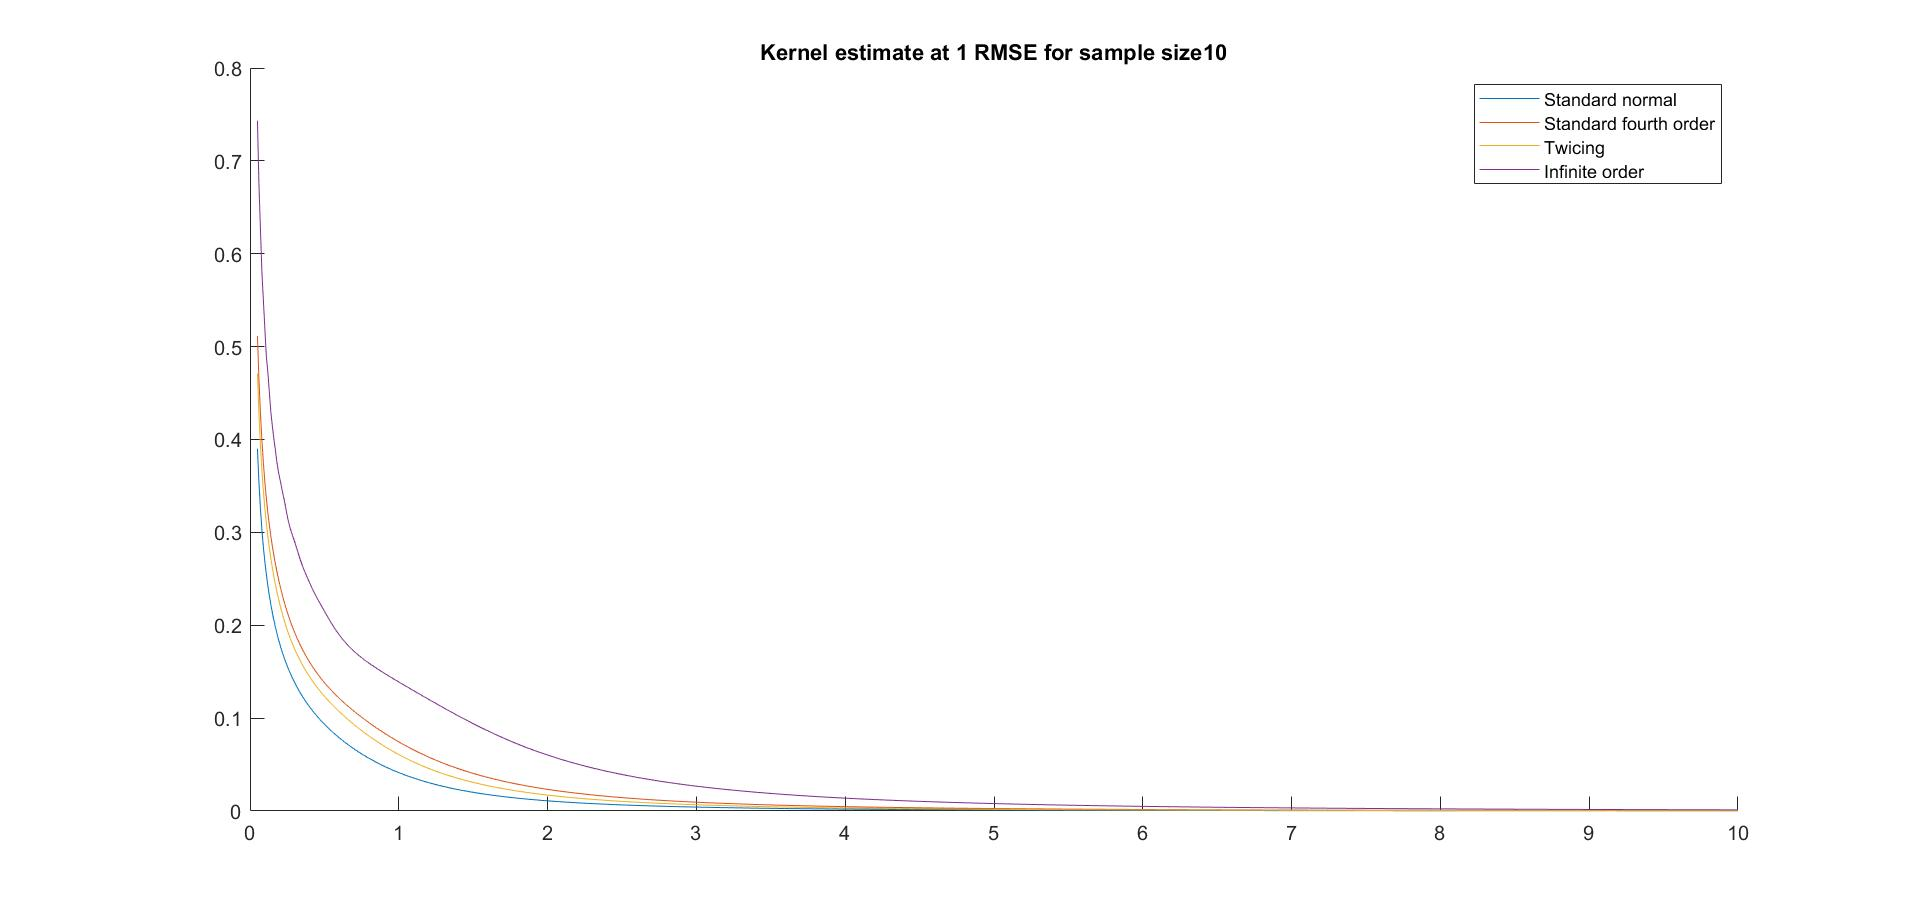
\includegraphics[width=13cm]{q2rmse10d.jpg}
\caption{Root mean square error of $\r{\hat{f}}(1)$ as a function of bandwidth for sample size 10.}
\label{fig:2rmse10}
\end{figure} 
\end{center}

\begin{center}
\begin{figure}
\centering
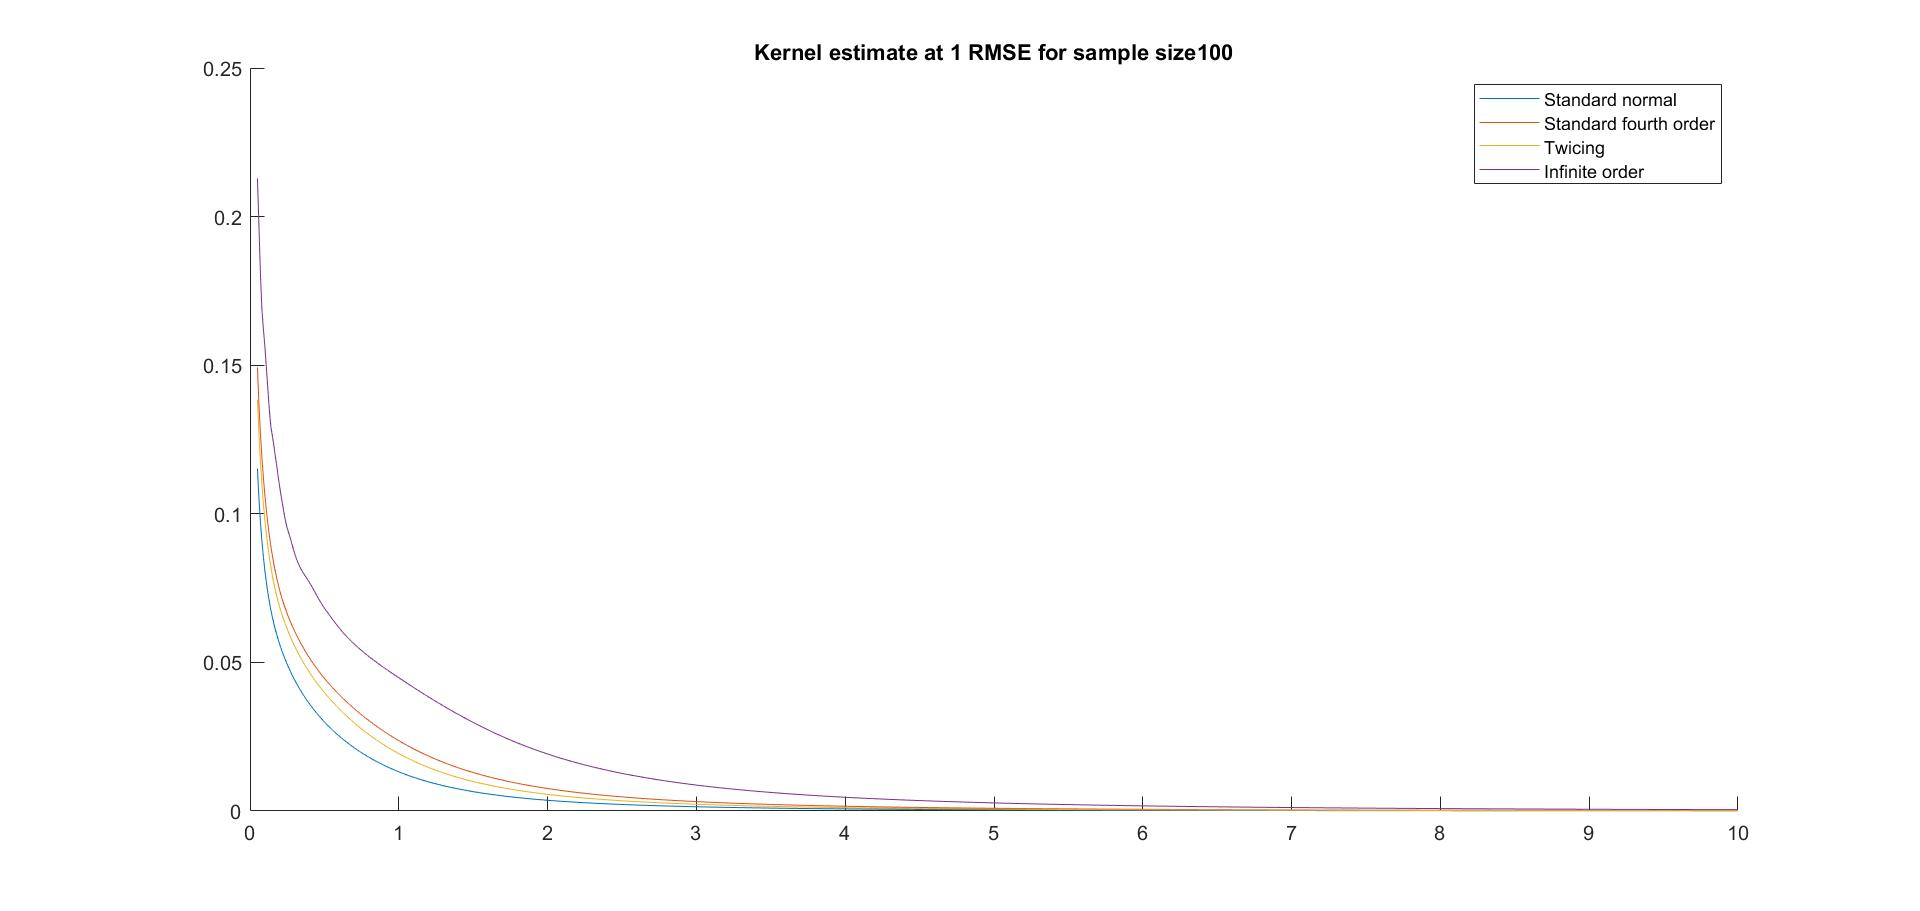
\includegraphics[width=13cm]{q2rmse100d.jpg}
\caption{Root mean square error of $\r{\hat{f}}(1)$ as a function of bandwidth for sample size 100.}
\label{fig:2rmse100}
\end{figure} 
\end{center}

\begin{center}
\begin{figure}
\centering
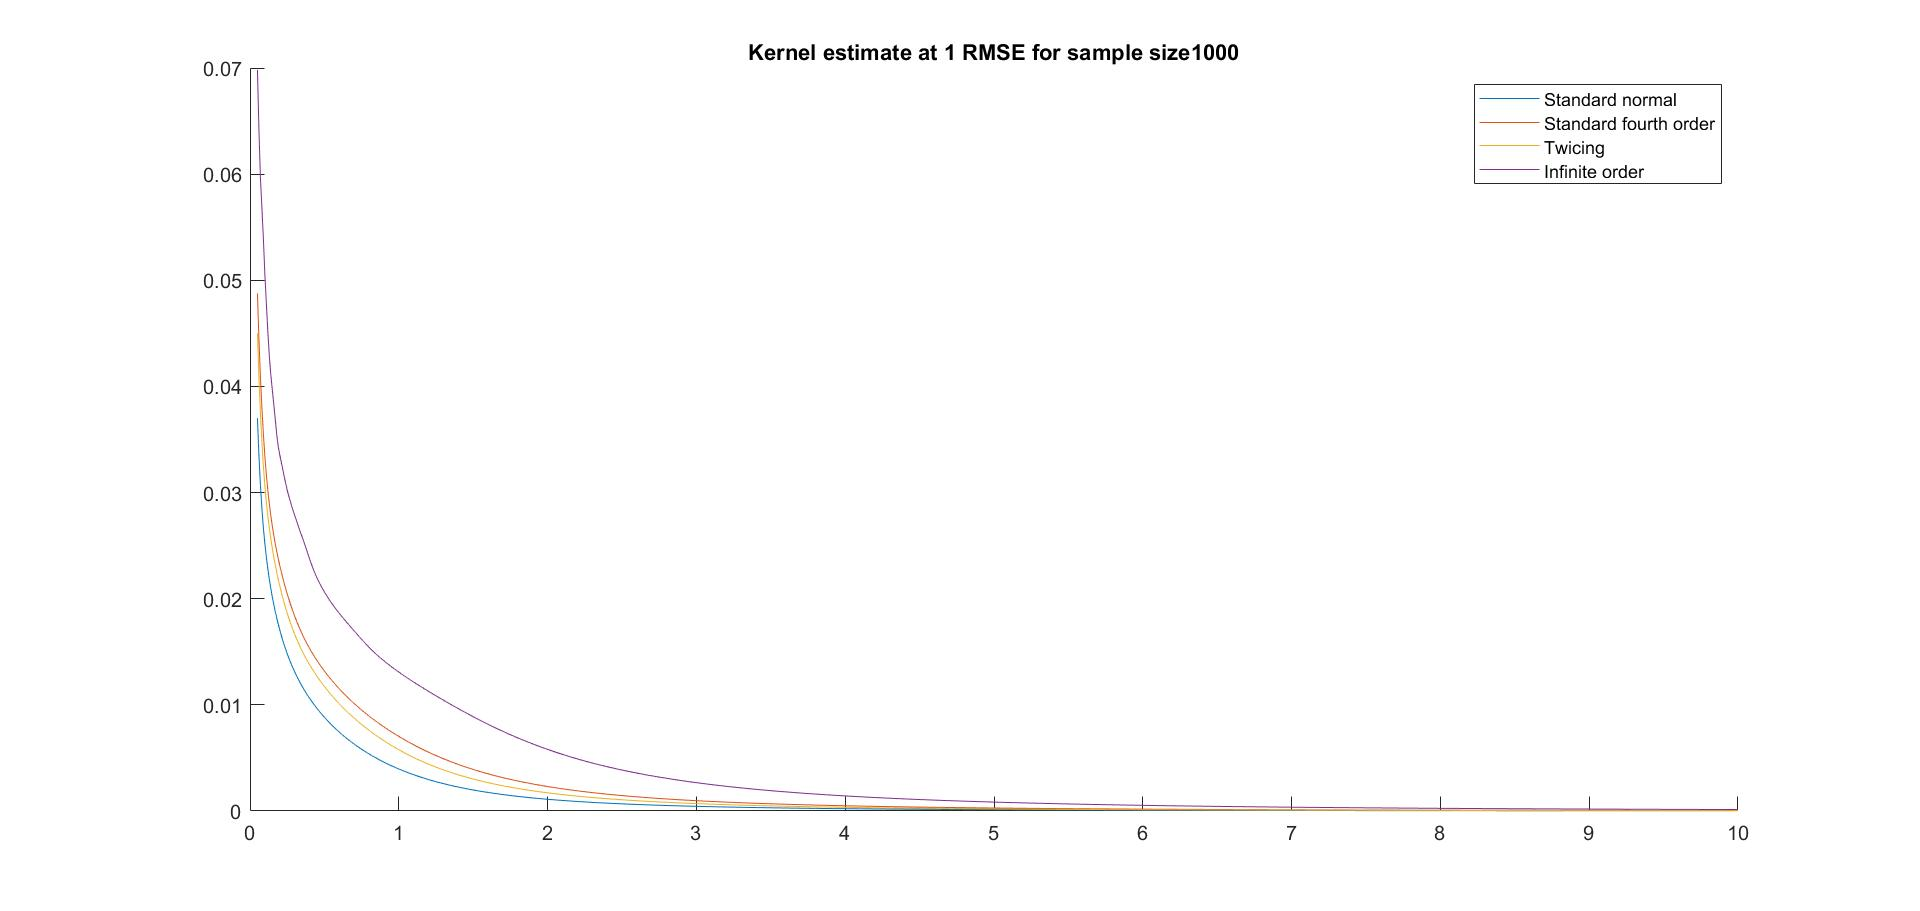
\includegraphics[width=13cm]{q2rmse1000d.jpg}
\caption{Root mean square error of $\r{\hat{f}}(1)$ as a function of bandwidth for sample size 1000.}
\label{fig:2rmse1000}
\end{figure} 
\end{center}



\subsection{Part (b).}
We subsequently use the previously generated data and the regression function 
\begin{equation} m(x)=\log(1+x^{2}),\end{equation}
to generate the data
\begin{equation} \r{y}_{i} = m(\r{x}_{i})+\r{u}_{i},\end{equation}
where we choose $\r{u}_{i}$ to be distributed as a standard normal. We again plot the root mean squared error against $h$, shown below. We note that this seems to be monotonic in $h$ for both the regression and density estimation, which I think indicates that I've not considered a wide enough range, or that I've done something wrong in the code. Either way, I have graphs and a short life, so, here we are. 

\begin{center}
\begin{figure}
\centering
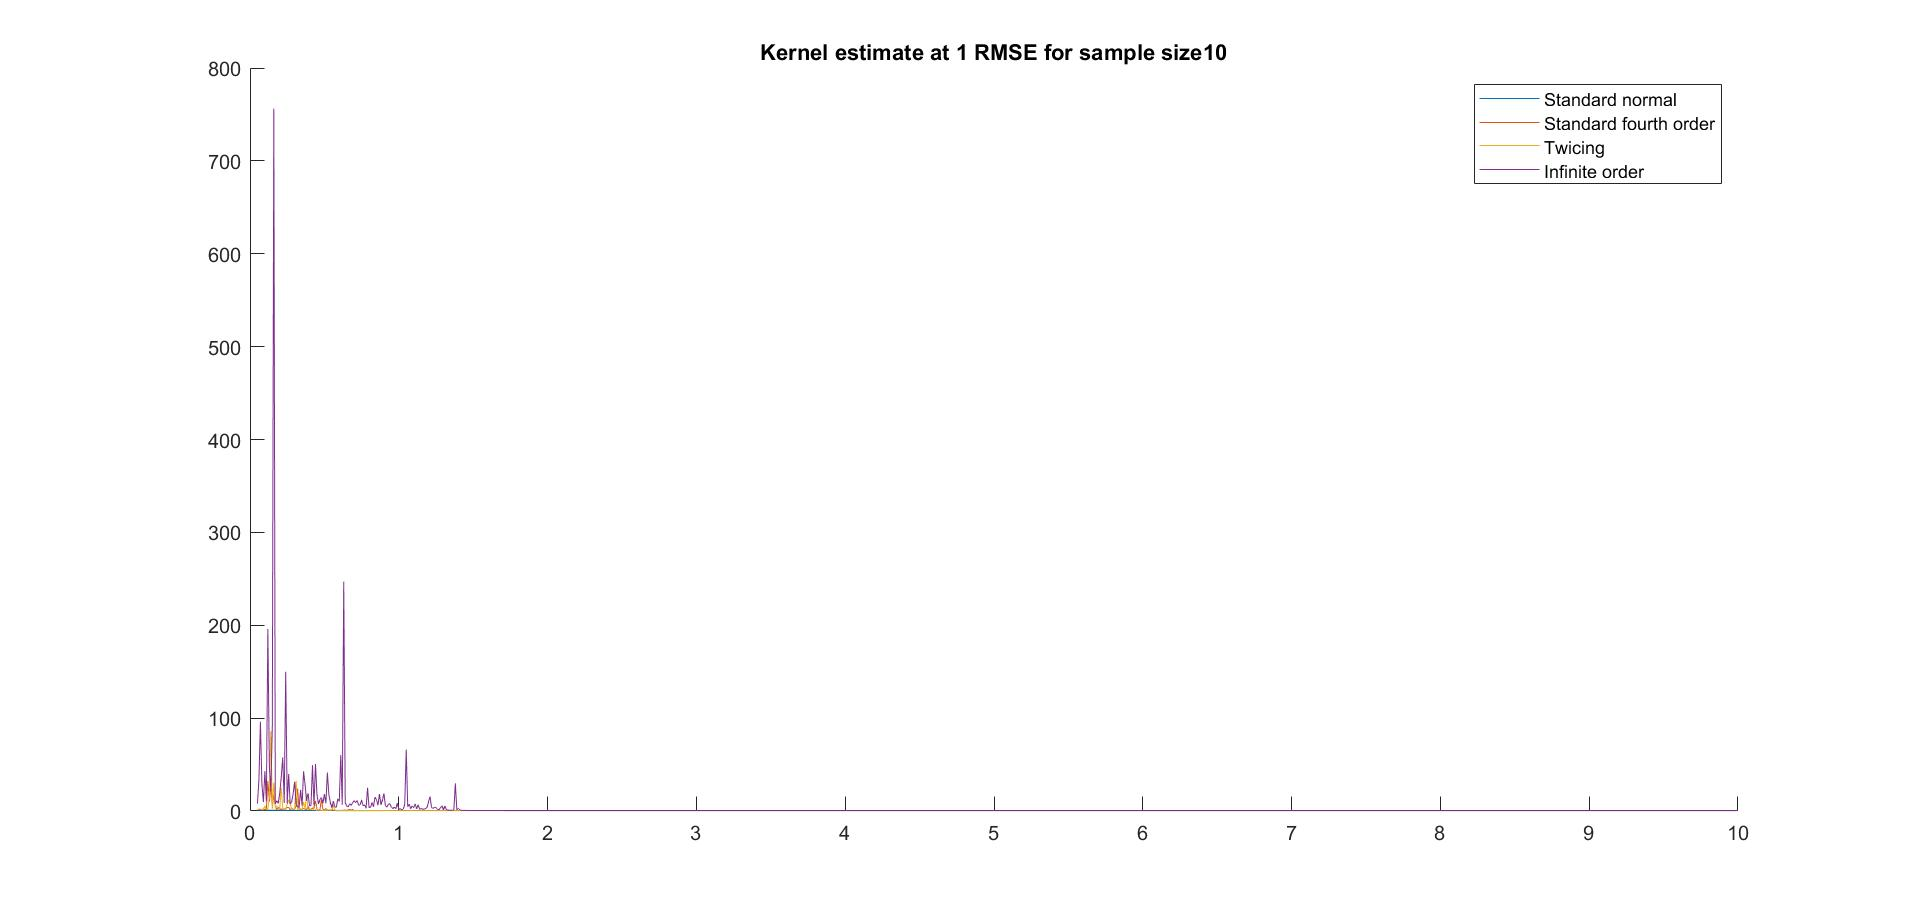
\includegraphics[width=13cm]{q2rmse10m.jpg}
\caption{Root mean square error of $\r{\hat{m}}(1)$ as a function of bandwidth for sample size 10.}
\label{fig:2rmse10m}
\end{figure} 
\end{center}

\begin{center}
\begin{figure}
\centering
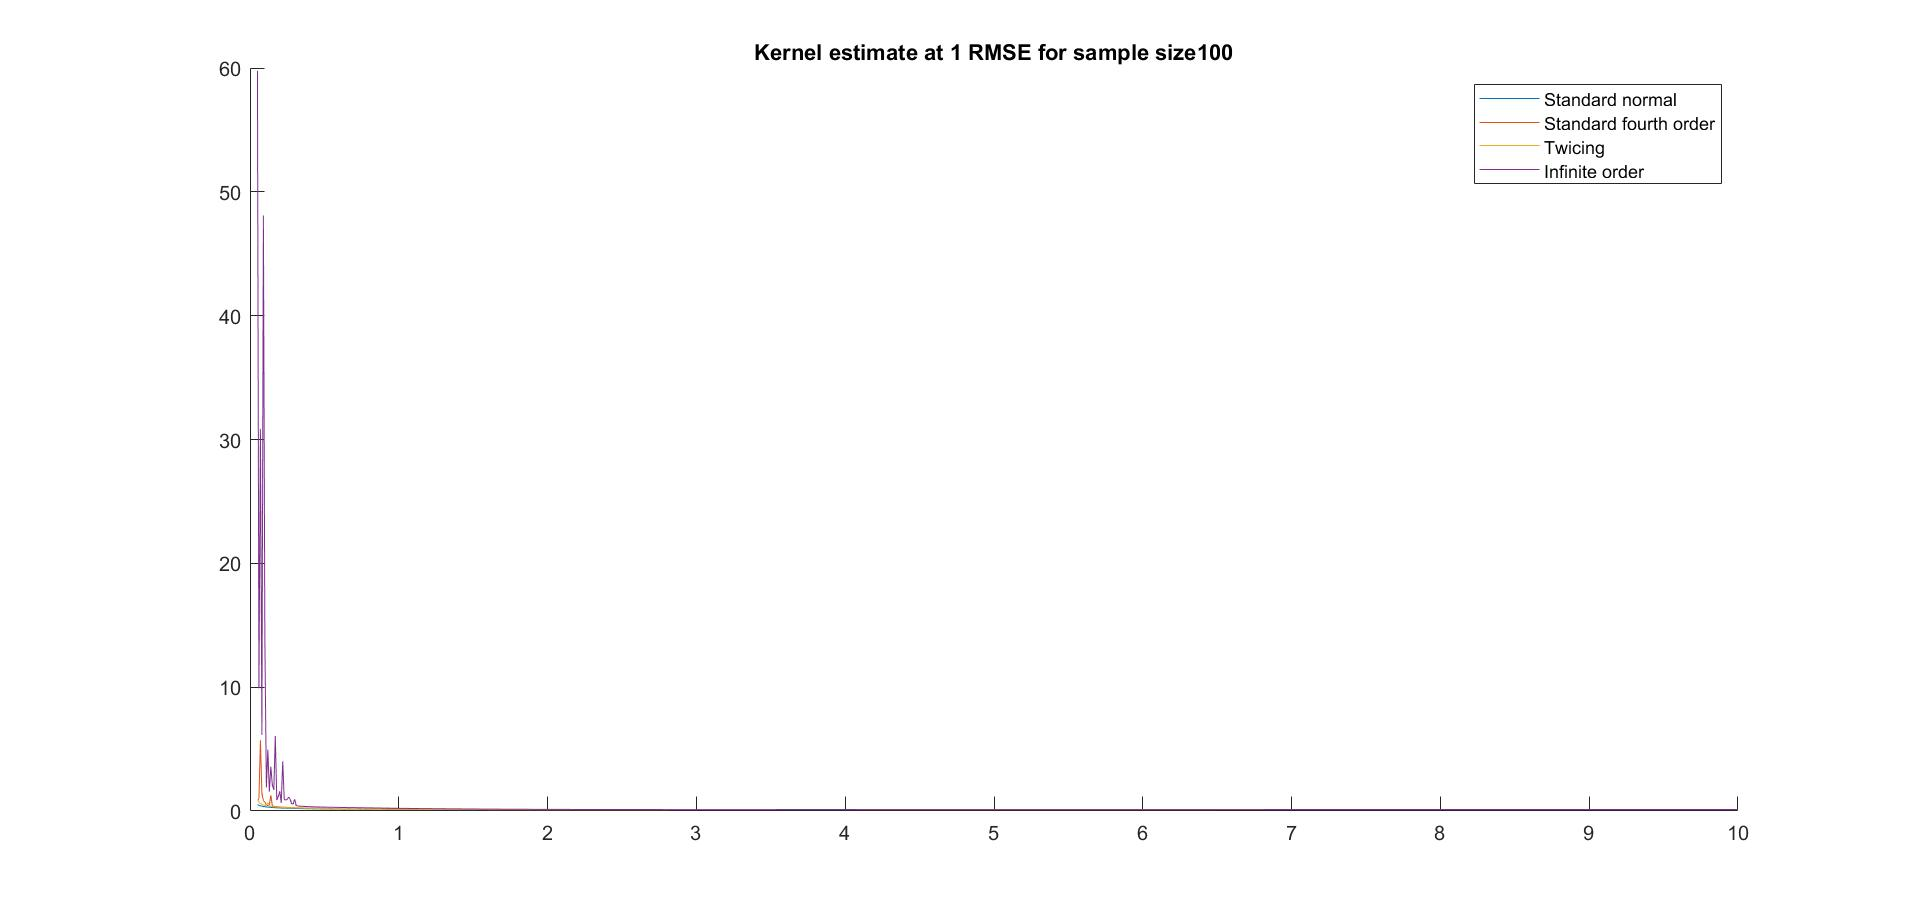
\includegraphics[width=13cm]{q2rmse100m.jpg}
\caption{Root mean square error of $\r{\hat{m}}(1)$ as a function of bandwidth for sample size 100.}
\label{fig:2rmse100m}
\end{figure} 
\end{center}

\begin{center}
\begin{figure}
\centering
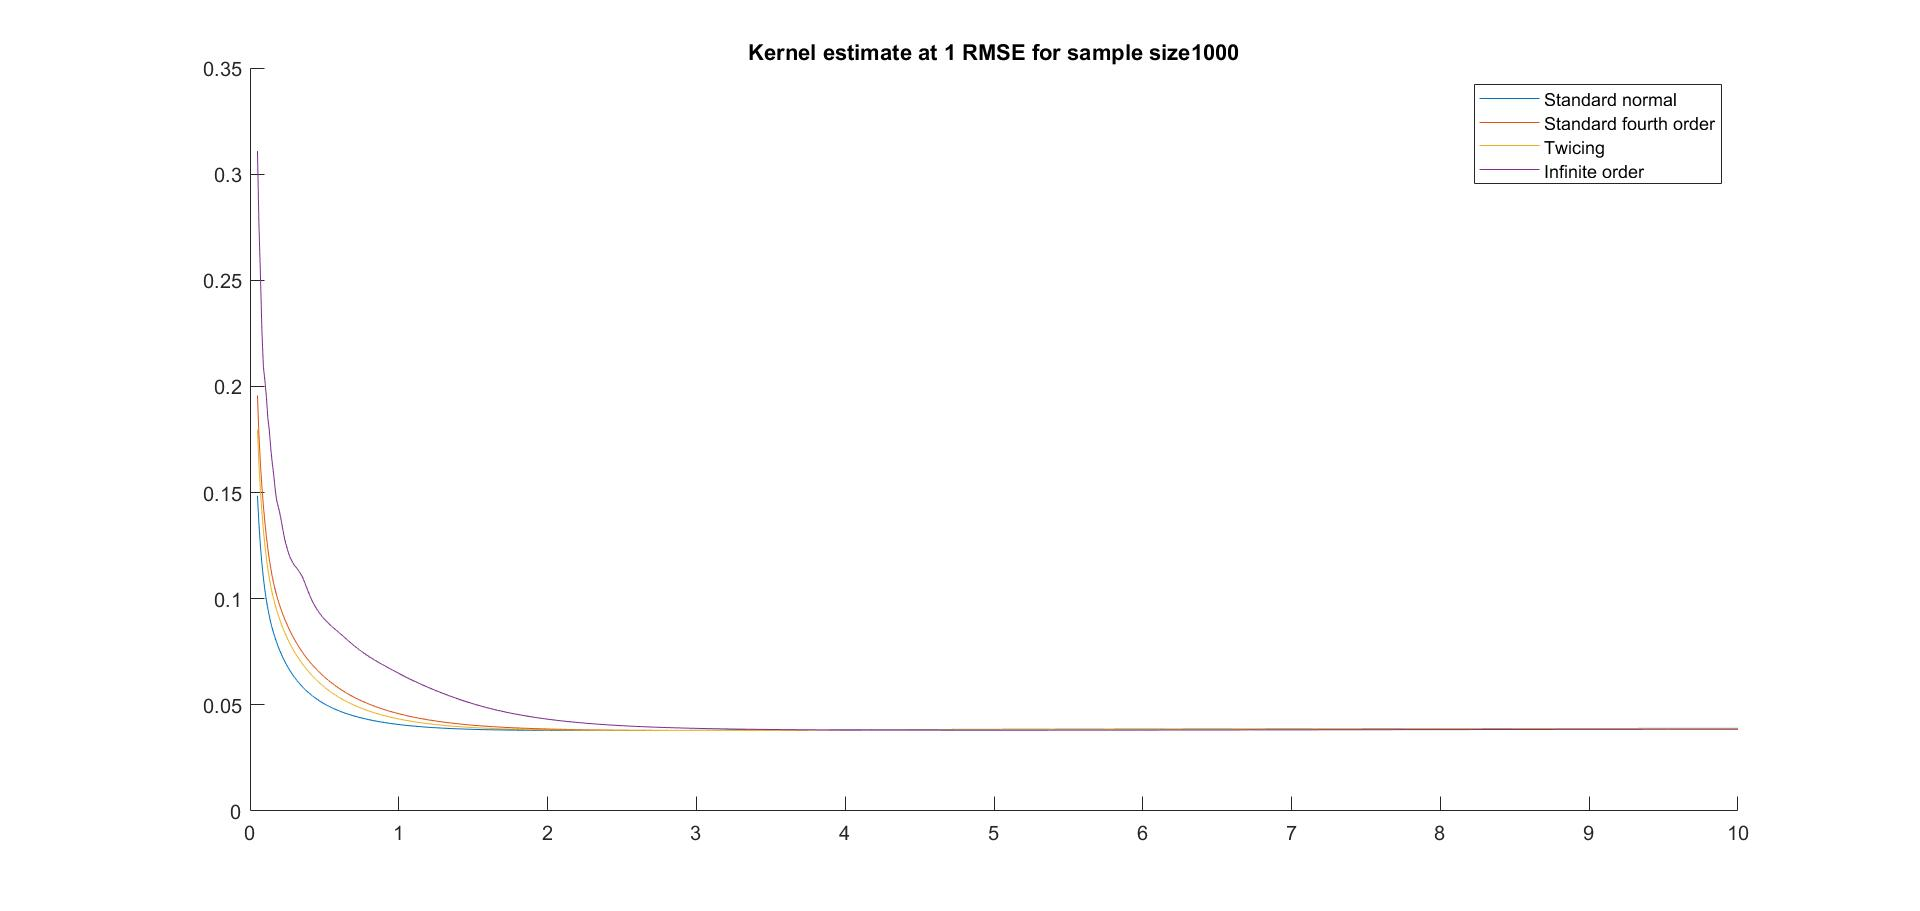
\includegraphics[width=13cm]{q2rmse1000m.jpg}
\caption{Root mean square error of $\r{\hat{m}}(1)$ as a function of bandwidth for sample size 1000.}
\label{fig:2rmse1000m}
\end{figure} 
\end{center}



\section{Question Three.}
\subsection{Part (a).}
We consider again a simulation using the standard Gumbel distribution, and consider two extremes for bandwidths, $h_{1}=10^{-6}$, and $h_{2}=10^{6}$. We use the standard normal kernel, presumably since there is evidence that the shape of the kernel is somewhat unimportant in determining the accuracy of the statistic \cite{trapp2012}. Using the same data set consisting of $n=1000$ observations, we plot the estimated distribution below for each bandwidth in Figure \ref{fig:q3d}.

\begin{center}
\begin{figure}
\centering
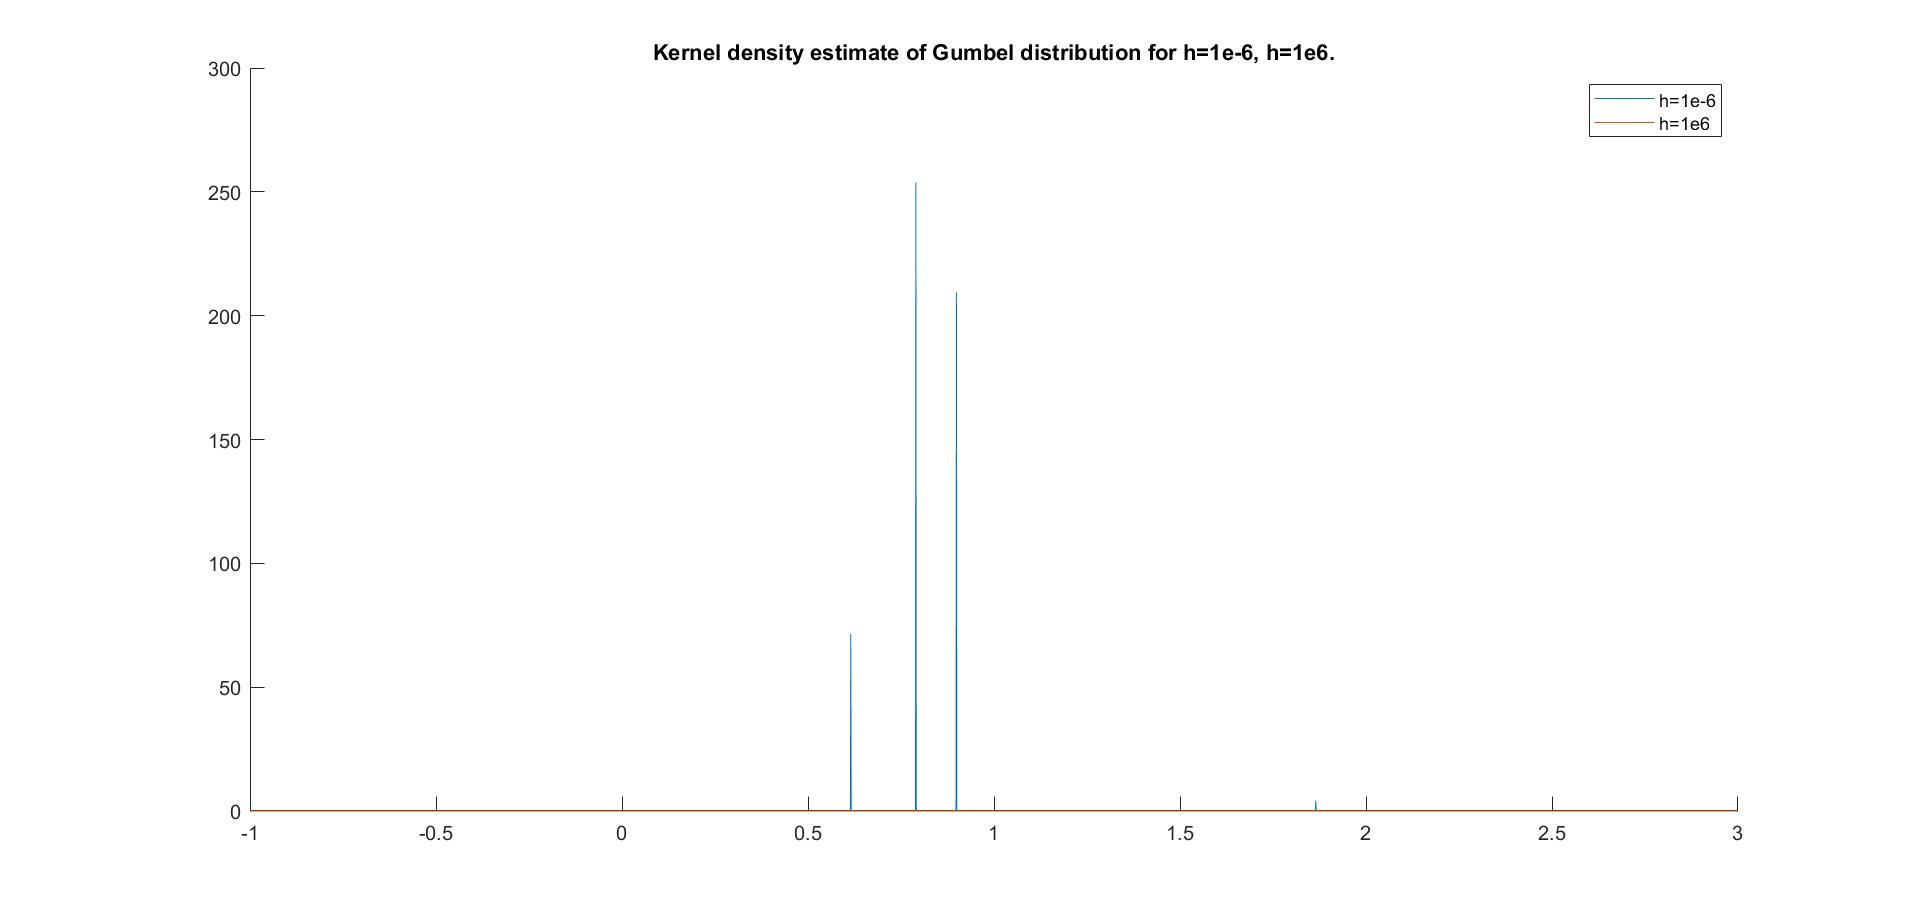
\includegraphics[width=13cm]{q3density.jpg}
\caption{Apparently the kernel estimator for the density of a standard Gumbel distribution. The kernel is the standard normal.}
\label{fig:q3d}
\end{figure} 
\end{center}

This is a mess, which I can only attribute to the absurd choices of bandwidths. I assume the spikes occur where the $x$ value is included in the sample.

For context, the Silverman bandwidth here is 0.3372.

\subsection{Part (b).}
As before, we do the same thing with the regressor $m$. This is plot in Figure \ref{fig:q3m}.

\begin{center}
\begin{figure}
\centering
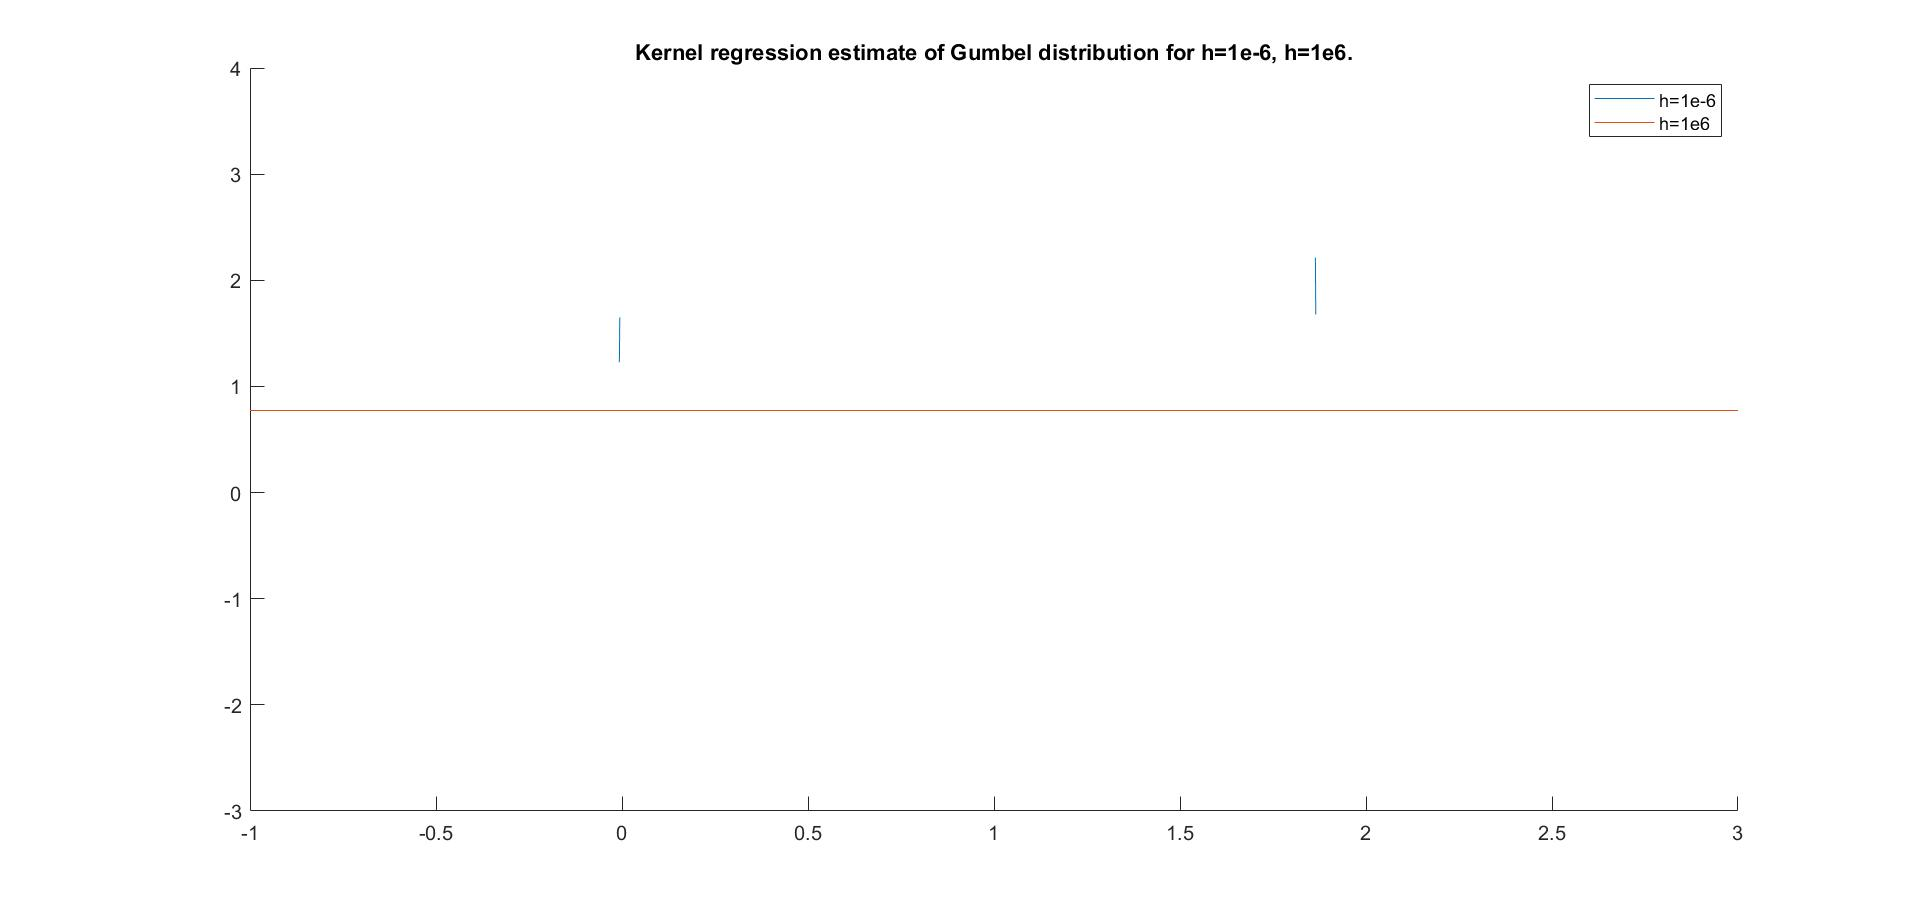
\includegraphics[width=13cm]{q3regression.jpg}
\caption{Apparently the kernel estimator for the regressor of a standard Gumbel distribution. The kernel is the standard normal.}
\label{fig:q3m}
\end{figure} 
\end{center}

This, clearly, is another mess.

\subsection{Part (c).}
Finally, we consider using Silverman's rule of thumb:
\begin{equation} \r{h_{s}} = \r{\hat{\sigma}}n^{-\frac{1}{5}}.\end{equation}
For our data set here, we get that $\r{h_{s}}=0.0725$. The plot of the density is given in Figure \ref{fig:q3u}. 

\begin{center}
\begin{figure}
\centering
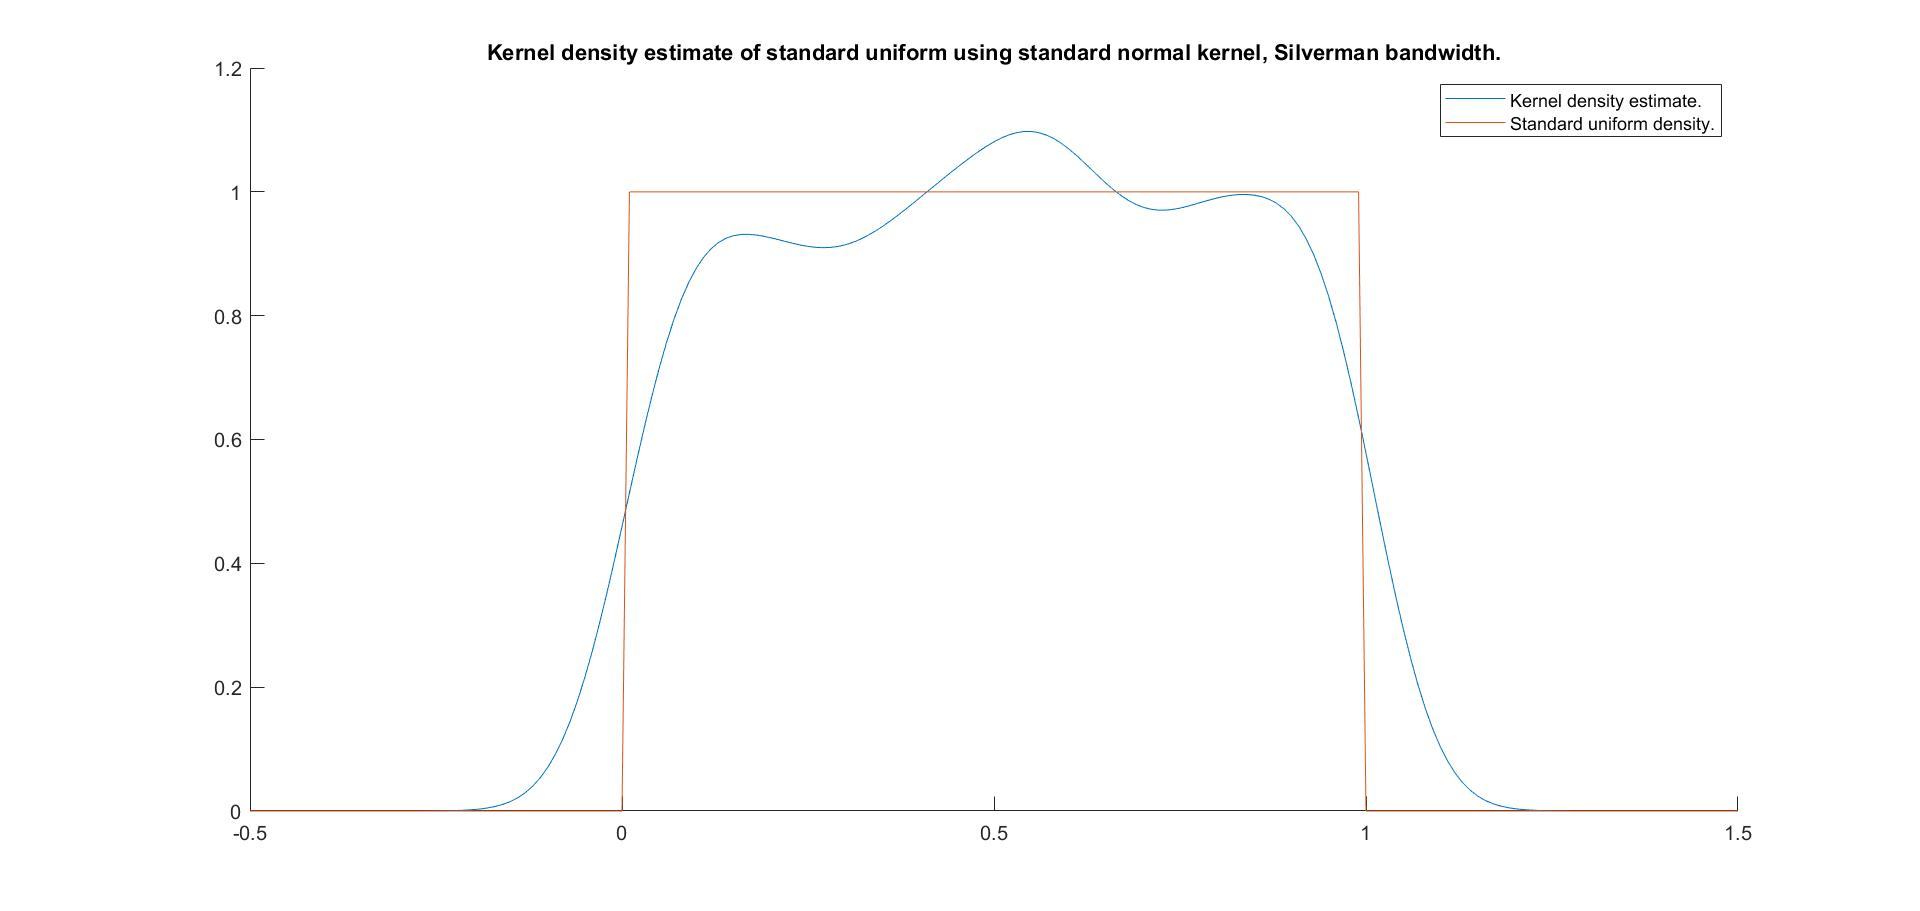
\includegraphics[width=13cm]{q3uniform.jpg}
\caption{The kernel density estimator of the standard uniform distribution with standard normal kernel and Silverman bandwidth.}
\label{fig:q3u}
\end{figure} 
\end{center}

We see that this fits much better, which is unsurprising, given the far more appropriate bandwidth.

\section{Question Four.}
\subsection{Part (a).}
My name is Ste. It begins with the letter `S.' So does the name of the state of South Carolina. We therefore look at income microdata from South Carolina in 2010 provided by the US census bureau. Throughout we use the standard normal kernel, and investigate options for bandwidth selection to construct a nonparametric estimation of the income distribution. 

We begin using Silverman's rule of thumb: $\r{h_{s}}=\r{\hat{\sigma}}n^{-\frac{1}{5}}$. We implement this on Matlab, which runs quickly enough that I don't have time to procrastinate somewhere else. The kernel estimator is plot in Figure \ref{fig:q4ks}. We note that the values are absurdly small (of the order $10^{-6}$) but this is not too concerning since the support of the distribution is very large.

\begin{center}
\begin{figure}
\centering
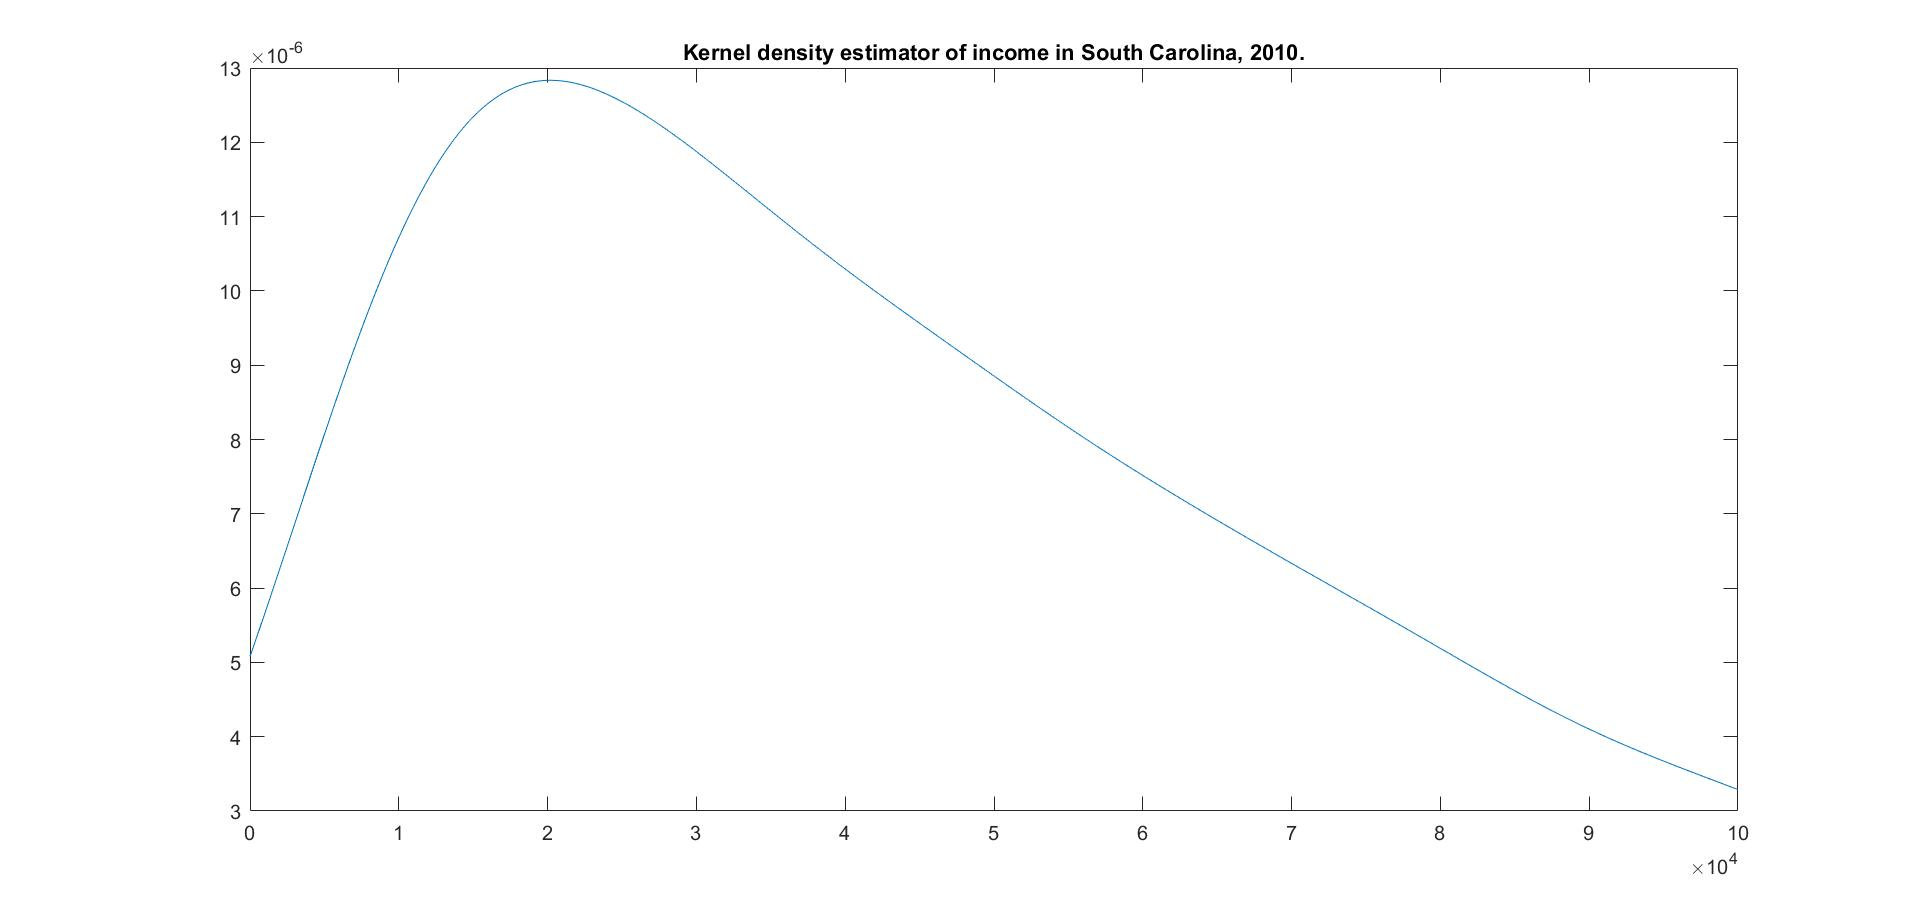
\includegraphics[width=13cm]{q4s.jpg}
\caption{The kernel density estimator of household income in South Carolina, 2010. The standard normal kernel is used, and the Silverman rule of thumb bandwidth, 0.0725 is used.}
\label{fig:q4ks}
\end{figure} 
\end{center}


\subsection{Part (b).}
We now use cross validation, which is to say, we choose $h$ to maximise 
\begin{equation} \sum_{i\leq n} \log\left\{\frac{1}{(n-1)h}\sum_{j\neq i}k\left(\frac{\r{x}_{j}-\r{x}_{i}}{h}\right)\right\}.\end{equation}
Our dataset (which we clean up with a few lines of code in Matlab), is somewhat large, consisting of over 19,000 observations. When we tried running this code in Matlab, we found that it ran far too slowly. 

We therefore migrated to c++ for the calculation of the cross-validated bandwidth. Despite the suggestion that classes would not be needed, it turned out that the easiest way to construct the objective that we need to maximise, it made sense to create a class consisting of a public array containing the data, and a public function that is the derivative of the objective (the derivative since we wrote non-linear solvers, a secant method and a bisection method. 

When we ran the secant algorithm, we found that while we could get the first order condition close to 0 (both positive and negative either side, so that, given the continuity of the function, we knew there was some finite root, and in fact at least two), the algorithm did not converge sufficiently quickly. We therefore identified a range on which a root had to exist by the intermediate value theorem, $[914,1200]$ (excluding negative bandwidths, though it's worth noting in passing that for the starting value -2871.93, the secant algorithm did actually converge fairly quickly). The bisection algorithm (set to a tolerance of $10^{-6}$) yielded the cross-validation bandwidth value 1059.4696. I'm surprised at how large this is, but it gives a somewhat reasonable curve, so fine\footnote{Sadly, I think this means I've wasted my time and the FOC that I wrote down is incorrect. Perhaps over the Fall break I'll have a second crack at it because I'm curious as to whether we'd expect the Silverman to perform better than the cross validation - I imagine not given that the latter is so much more expensive.}. The added lumpiness is an effect of the larger bandwidth, since the estimator is relying on data points further out from each $x$.  The kernel estimator is plot in Figure \ref{fig:q4c}.

\begin{center}
\begin{figure}
\centering
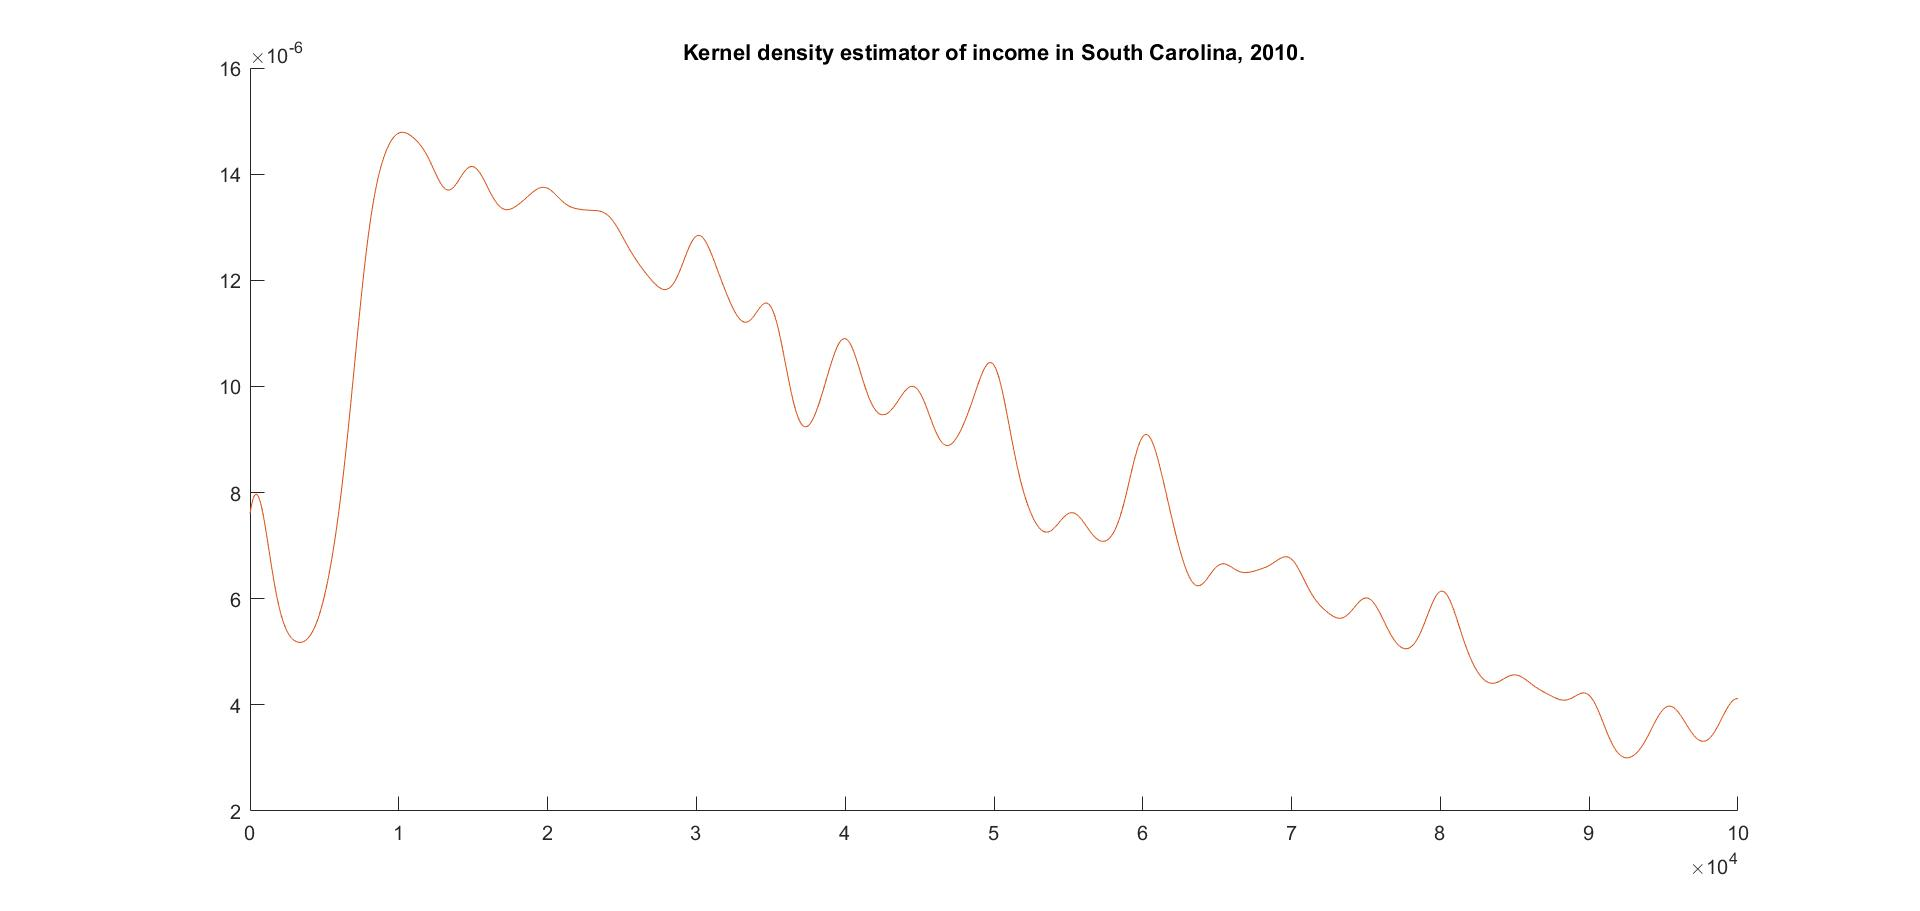
\includegraphics[width=13cm]{q4c.jpg}
\caption{The kernel density estimator of household income in South Carolina, 2010. The standard normal kernel is used, and the cross-validation bandwidth 1059.4696 is used.}
\label{fig:q4c}
\end{figure} 
\end{center}



\section{Question Five.}
We are asked to find three examples of applied papers employing kernel regression. Because I'd rather our world isn't such that my children or grand children will have to kill someone for a bottle of water, I have somewhat of an interest in economics relating to climate change, so that's the bent with which I took this task. An exceedingly brief summary of each paper is provided.

\subsection{Nonparametric modeling of carbon prices, J. Chevallier (2011)\cite{chevallier2011}.} 
Chevallier applies a standard local linear regression approach to the problem of carbon prices (for example, the EU ETS), with a multiplicatively separable and symmetric kernel and scalar bandwidth. He does this by using the model
\begin{equation} \r{y}_{t} = \mu(\r{x}_{t-1})+\sigma(\r{x}_{t-1})\r{\varepsilon}_{i},\end{equation}
where $\r{x}_{t}$ consists of an appropriate number of lagged $\r{y}$ values, $\r{y}_{t}$ is the carbon price at time $t$, and $\r{\varepsilon}_{t}$ is some shock. He contrasts this to the approach common in the literature which is to assume $\mu$ and $\sigma$ are linear functions.  

It is notable that this model is nonparametric both in the lack of assumptions on $\mu$ and $\sigma$, but also that the number of lags contained in $x$, denoted by $m$, is unknown. This is chosen as a tuning parameter along with (as is of course standard) the bandwidth of the kernel. The lack of constraints on $m$ (barring a maximum value $M$) is interesting in this case since this affects the dimensionality of the estimator. To approach this, Chevallier creates an error function which one optimises over $h$ \textbf{and} $m$. This error function (the ``asymptotic final prediction error,'' as the paper is constructed with a view to forecasting) involves coefficients that depend on unknown densities, and hence must also be approximated nonparametrically.

The take home of the paper is that the nonparametric model offers greater forecasting and expository power than does the linear models standardly assumed in the literature. 


\subsection{The polarization of American environmental policy: A regression discontinuity analysis of Senate and House votes, 1971-2013, S.E. Kim \& J. Urpelainen (2017)\cite{kim2017}.}
For all it's pros and cons, the two-party system leads to an environment suitable for regression discontinuity design, since the binary independent variable for the purpose of much analysis - the party of the legislator in a given constituency - is an indicator function:
\begin{equation} \mathds{1}\{V_{p}>0.5\},\end{equation}
where $V_{p}$ denotes the share of votes for party $p$. 

Kim and Urpelainen exploit this fact to use an RDD approach to examine whether party membership is an explainer of voting on environmental legislation independent of electoral conditions in the United States. They do this in two ways: a parametric approach that uses lags on electoral results on an assumed functional form for votes on evironmental bills (not of interest for our purposes), and a nonparametric RDD approach.

The key insight (taken from other authors) is that for close races - `close' eventually being defined in the paper as within 0.5\%, a value that is able to be so small due to the massive amount of observed votes (319,258) - the selection of a legislator is effectively random, and hence is a quasi-experimental environment. Intuitively, this is explained by the fact that in such seats, the decision is made by a handful of votes, and an individual voter's turnout is influenced by random variables - the example in the paper being the weather, though the argument is more convincing when one considers individual heterogeneity in voter turnout, such as how ill an individual may be feeling, the amount of fuel in the car and the price of fuel on the day, or any other such real-world concern. The authors provide evidence that districts that are marginal are often similar in terms of explanatory variables such as income, thus strengthening their ``almost-random'' (their words) assumption. One should note - and they do - that a possible driver for elections in marginal seats is in fact heterogeneity in the candidates that is independent of political affiliation, such as their career history, but the authors control for this by excluding samples where there is a large discrepancy in the characteristics of the candidates in a given election. They have an absolutely massive data set which I guess makes the decision to do that a fairly easy one.

The ultimate conclusion of this paper is that the polarisation of party elites on environmental policy is precisely that, and not reflective of the degree of public polarisation. That is, all things equal, a Republican will vote to subsidise polluters to protect local industry, but will vote against subsidies to green energy because that's `interfering with the market.' This is tested for a variety of subsamples differentiated by factors such as geography, and in all cases, the House is separated from the Senate, due to the perception of the Senate as acting in a less partisan manner, presumably due to less frequent electoral pressures. 


\subsection{Carbon dioxide emissions and governance: A nonparametric analysis for the G-20, G.E. Halkos, G.N. Tzemerez (2013)\cite{halkos2013}.}
Halkos and Tzemerez present a somewhat rudimentary analysis that links World Bank indicators of governance (of which there are six, concentrating on different aspects of governance, such as citizen participation, rule of law, etc.) and carbon emissions for the G20 countries, from 1996 to 2010. This is done using a Nadaraya-Watson estimator for
\begin{equation} g(x) = \E[\r{y}_{i}|\r{X}_{i}=x],\end{equation}
where $x$ is the vector of governance indices and $\r{y}_{i}$ is CO$_{2}$ emissions. The units are countries and year, which I would have thought threw up some fixed effects issues but those don't seem to be discussed.

I won't deny the similarity of the approach in this paper to the approach in the first paper I've offered, but I believe the differences are significant enough. For one, the first paper is more sophisticated in that it offers the nonparametric kernel treatment to functions in a stochastic process in discrete time rather than simply a regressor function, and also in that by incorporating uncertainty in the appropriate number of lags $m$, they extend the nonparametric analysis in a novel way, including the construction of a new process for selecting bandwidth. By contrast, this paper simply applies the NW estimator, and uses cross-validation to determine the bandwidth. However, to be fair to this paper, while the first paper offered uses a scalar bandwidth, this paper uses a vector bandwidth for multivariate kernel estimation (though it is just a diagonal matrix).

Looking at the graphs, it's not clear that they draw any useful conclusions. They observe that the regressions they obtain are highly nonlinear, but they are also not monotonic or really immediately recognisable as a function driving data as opposed to just noisy waves. No offence to Halkos and Tzemerez, but I'd be highly surprised if they ended up reading my assignment for a second year class anyway.



\section{Question Six.}
We run a simulation exercise on a binary choice model:
\begin{equation} \r{y}_{i} = \mathds{1}\{G(\r{x}_{i}'\theta_{0})+\r{u}_{i}\geq0\},\end{equation}
where $G$ is a linking function, and $\r{u}$ is noise. For simplicity, we take $G$ to be the identity mapping. This actually doesn't help our results however - it would seem I suck at coding. We consider a sample of 1000 individuals with five characteristics, the first two of which are discrete, the final three of which are continuous. 

Not that I think it should matter, but, the first is distributed Poisson with parameter 3, the second is uniform on $\{-10,-9,\cdots,9,10\}$, the third is an exponential with parameter 3, the fourth is uniform on $[-10,10]$, and the final is distributed as a standard normal. 

Normal errors are distributed either homoscedastic with variance $1$, and normal errors with homoscedastic variance have variance $e^{x_{5}}$. Non-normal errors are distributed as a fifty-fifty chance of being drawn from a normal with mean -1 and a normal with mean 1, where for the homoscedastic errors, these normals have variance 1, and for heteroscedastic errors, they have variance $e^{x_{5}}$. While this is built from normals, we feel that the bimodal nature of the distribution makes it suitably different from a normal for the purpose of adding errors.

We run each of these possibilities with $n=100$ and $n=1000$. We consider the probit estimator, the average derivative estimator, the Klein-Spade estimator, and the maximum score estimator. For the Klein-Spade estimator, we use a standard normal kernel with the Silverman bandwidth for $\vec{\r{X}}\theta$, where $\theta$ is the parameter of the objective. For the average derivative estimator, we use a product of standard normal kernels, and for the bandwidth, select the Silverman bandwidth fro $\vec{\r{X}}\r{\hat{\theta}_{KS}}$, where $\r{\hat{\theta}_{KS}}$ is the Klein-Spade estimator.

The squared error (the difference with the true value of $\theta_{0}$, which is $(-16,-8.8,1.87,18.3,1)'$) is reported for each simulation. I'll be honest, the main two take aways from this is that they all suck (I think computing a decent bandwidth is tricky but I'm not sure why probit is so lame when it's exactly the probit model), and that you should never do anything with kernels in Matlab, and if I ever program a nonparametric thing again, you can bet your bottom dollar that I'll be writing it in c++. The table below is the squared errors divided by 1000 (note then that 0s represent only that the error was less than 1), though that's a hell of a lot better than most.
\begin{center}
\begin{tabular}{|c||c|c|c|c|}
\hline 
&Klein-Spady&Probit&Maximum score &Average derivative \\ \hline \hline
1&    0.0233  &  0.0250 &   0.0261 &   0.0578 \\ \hline
2&   0.0137 &   0.0041 &   0.0214 &   0.5009 \\ \hline
3 &      0   &      0  &  0.0261 &   0.0594 \\ \hline
4 &      0   &      0 &   0.0214 &   1.0804 \\ \hline
5 &      0   &      0  &  0.0261 &   0.0594 \\ \hline
6 &      0   &      0  &  0.0214  &  0.6824 \\ \hline
7 &      0   &      0  &  0.0261  &  0.0578 \\ \hline
8 &      0   &      0  &  0.0214  &  0.8278 \\ \hline
\end{tabular}
\end{center}


\section{Question Seven.}
\subsection{Part (a).}
We consider an RDD estimator using standard kernel regression estimation, so that the parameter is an estimate of the difference of the regression estimators either side of the treatment cutoff. Since the Nadaraya-Watson estimator is upward biased if the conditional expectation $m$ is upward sloping at the boundary \cite{racine2001}\cite{cunha13}, we have that the difference would be exaggerated, and hence the RDD estimate is upward biased.

\subsection{Part (b).}
Beyond new kernel's and new estimators, the only change we can make is to the data, and hence we consider transformations of the data that will reduce the boundary bias. 

Our intuition as to why the boundary bias occurs for the kernel distribution estimator is that the estimator ``expects'' there to be data to both sides of the boundary point, and finding only half as many points as it expects, and hence introduces bias. One method to deal with this could be to add points to the other side of the estimator to make up for this, with the most intuitive choice of points being a reflection of the existing data. In fact, such an approach is taken by Hall and Wehrly (1991), who find using a simulation study that an estimator that reflects data across boundaries and runs as a standard kernel estimator outperforms common boundary-corrected kernels, and performs approximately as well as estimators proposed by Gasser-Muller \cite{hall1991}.



\section{Question Eight.}
We consider the partially linear model
\begin{equation} \r{y}_{i} = \r{x}_{i}'\theta_{0}+g(\r{z}_{i})+\r{u}_{i}.\end{equation}
The Robinson estimator replaces the structural equation with
\begin{equation} \r{y}_{i}-\r{\bar{y}}=(\r{x}_{i}-\r{\bar{x}})'\theta_{0}+g(\r{z}_{i})-\r{\overline{g(z)}}+\r{u}_{i}-\r{\bar{u}},\end{equation}
and runs OLS on this. The other estimator, which shall hereafter be the Wren estimator (named after my cat, because it's late, and I need to give this thing a name), replaces the structural equation with
\begin{equation} \r{y}_{i}-\r{y}_{i-1}=(\r{x}_{i}-\r{x}_{i-1})'\theta_{0}+(g(\r{z}_{i})-g(\r{z}_{i-1}))+(\r{u}_{i}-\r{u}_{i-1}),\end{equation}
where observations are ordered by $\r{z}_{i}$, and runs OLS on this. It can be shown that the Robinson estimator, $\r{\hat{\theta}_{R}}$ is
\begin{equation} \r{\hat{\theta}_{R}} = \theta_{0}+(\r{\Delta \vec{X}}'\r{\Delta \vec{X}})^{-1}\r{\Delta \vec{X}}\r{\Delta g(\vec{Z})}+(\r{\Delta \vec{X}}'\r{\Delta \vec{X}})^{-1}\r{\Delta \vec{X}}'\r{\vec{u}},\end{equation}
where
\begin{equation} \r{\Delta \vec{X}} = \r{\vec{X}}-\r{\bar{\vec{X}}}\vec{1},\end{equation}
where $\vec{1}$ is a vector of 1s; and that the Wren estimator $\r{\hat{\theta}_{W}}$ is
\begin{equation} \r{\hat{\theta}_{W}} = \theta_{0} + (\r{\vec{X}_{-1}}'\r{\vec{X}_{-1}})^{-1}\r{\vec{X}_{-1}}\r{g(\vec{Z})_{-1}} + (\r{\vec{X}_{-1}}'\r{\vec{X}_{-1}})^{-1}\r{\vec{X}_{-1}}\r{\vec{u}},\end{equation}
where subscript -1 denotes a lagged value.

Note that we can consider $\Delta$ to be a matrix
\begin{equation} \vec{I} - \frac{1}{n}\vec{1}_{n\times n},\end{equation}
so that 
\begin{equation} \r{\Delta \vec{X}} = \Delta\r{\vec{X}}.\end{equation}
Similarly, if we write 
\begin{equation} \vec{L} = \vec{I} - \vec{I}_{-1},\end{equation}
where $\vec{I}_{-1}$ is the identity matrix with all entries shuffled 1 to the left, we can write
\begin{equation} \r{X_{-1}}=\vec{L}\r{\vec{X}}.\end{equation} 

The intuition of the success behind each of these estimators is that in the structural equations, the bigger $n$ is, the smaller the differenced $g(z)$ term is. For the Wren estimator, we see that as $n$ grows larger, since the observations are ordered by $\r{z}$, the closer each $\r{z}_{i}$ is to its neighbour, and hence, for sufficiently large $n$ and not awful $g$, the closer each $\r{g}(\r{z}_{i})$ is to its neighbour, and hence the lower the error added to the estimator. It is however very hard to determine as a function of $n$ what the average distance between neighbour points is, or maybe I just don't know enough about order statistics, but trying to integrate directly from the joint pdf of order statistics the expectation of $|\r{z}_{i}-\r{z}_{i-1}|$ is very, very hard. I am going to point out this note by Lopez (2011), which indicates the problem is certainly not a trivial one, as work in 2011 was still being done to find upper bounds on expectations of differences between order statistics even given strict assumptions regarding the support of the distribution \cite{lopez2011}.

We also note here, while we're discussing the errors of $\r{\hat{\theta}_{W}}$ that the errors in the structural equation inherit the iid property from the underlying data, and hence is simply white noise.

It is not actually clear to me why the second term in $\r{\hat{\theta}_{R}}$ would disappear now that I'm looking at it, except perhaps if there are hopes of orthogonality between $\r{x}$ and $\r{z}$.



\section{Question Nine.}
We are asked to consider the advantages of the median absolute deviation as a measure of the success of an estimator in simulation studies over the root mean squared error. The definition of the median absolute deviation (hereafter MAD) is defined\cite{leys2013} as
\begin{equation} \text{MAD} = \text{median}\left(\r{x}_{i}-\text{median}(\r{x}_{i})\right).\end{equation}
That is, it is the median of the distribution of the data minus the median of the data. The first thing to note of this estimator is that the population analogue of this exists for all distributions (since every distribution has a median), which allows an economist to choose simulation data from a wider variety of distributions, no longer restricted to moment concerns.

Perhaps more importantly is the robustness of the measure to outliers. This is obvious intuitively, since individual observations cannot effect the median, which enters the formula twice (offering two layers of `protection' from rogue observations). If we define the notion of a breakdown point as the number of observations that are allowed to go to infinity before a statistic describing spread goes to infinity, it is clear that the root mean square error has a breakdown value of 0\cite{leys2013}, whereas the median has a breakdown value of $\frac{n}{2}-1$, which is a significant improvement, and indicates much greater robustness to outliers, which are often not of interest in simulation exercises.


\section{Question Ten.}
We consider $\r{x}_{i}$ drawn i.i.d. from $N(\theta_{0},1)$ with $\theta_{0}\in\{0,1,\cdots,10000\}$, and consider the rates of convergence of the sample mean and the MLE. We presume that the intention of this is for the sample mean to be simply the sample mean (i.e. so that $\r{\bar{\theta}}\not\in\Theta$), whereas the MLE is the maximiser of the log likelihood over $\Theta=\{0,1,\cdots,10000\}$. Note that since in a continuous parameter space we have 
\begin{equation} \r{\hat{\theta}_{MLE}}=\r{\bar{\theta}},\end{equation}
this is the only way to consider them as separate estimators, and because the log likelihood for a normal distribution of known variance is nicely behaved, we have that for the discrete (in fact finite, which is important in the paper I'll reference) parameter space, that
\begin{equation} \r{\hat{\theta}_{MLE}}=[\r{\bar{\theta}}],\end{equation} 
where $[\cdot]$ is the rounding operator which maps $\cdot$ to the nearest integer.

The rate of convergence of the MLE comes from the argument from Choirat et al (2012) which demonstrates for m-estimators in general - with MLE given as a particular example - have convergence rate
\begin{equation}\label{eqn:rate} \frac{e^{-cn}}{n^{\frac{1}{2}}},\end{equation}
where $c$ is some positive constant expression of parameters introduced in the proof \cite{choirat2012}. The convergence rate of the sample mean is, as is standard since we are calculating it as though the parameter space is continuous, $\sqrt{n}$.

We also conduct a simulation exercise, generating 1000 data points from $N(326,1)$ (the number of seats technically needed for a majority in the House of Commons, excluding seats held by the Speaker and their Deputies, and seats formally held by abstaining Sinn Fein members) and compare the sample average (continuous) to the MLE (discrete) by plotting the estimates against number of observations to observe how much better the MLE performs. We do this rather than report the root mean squared error of multiple simulations as we expect that for any reasonable $n$, the value of $\r{\hat{\theta}_{MLE}}$ will be $\theta_{0}$ and return a root mean squared value of 0 (of course indicative of greater performance, but not particularly worth running simulations for). Since the variance is small compared to the gap between possible $\theta$s in the question given, we increase the variance to 100 for the purpose of our simulation, and to 10. 

\begin{center}
\begin{figure}[!htb]
\centering
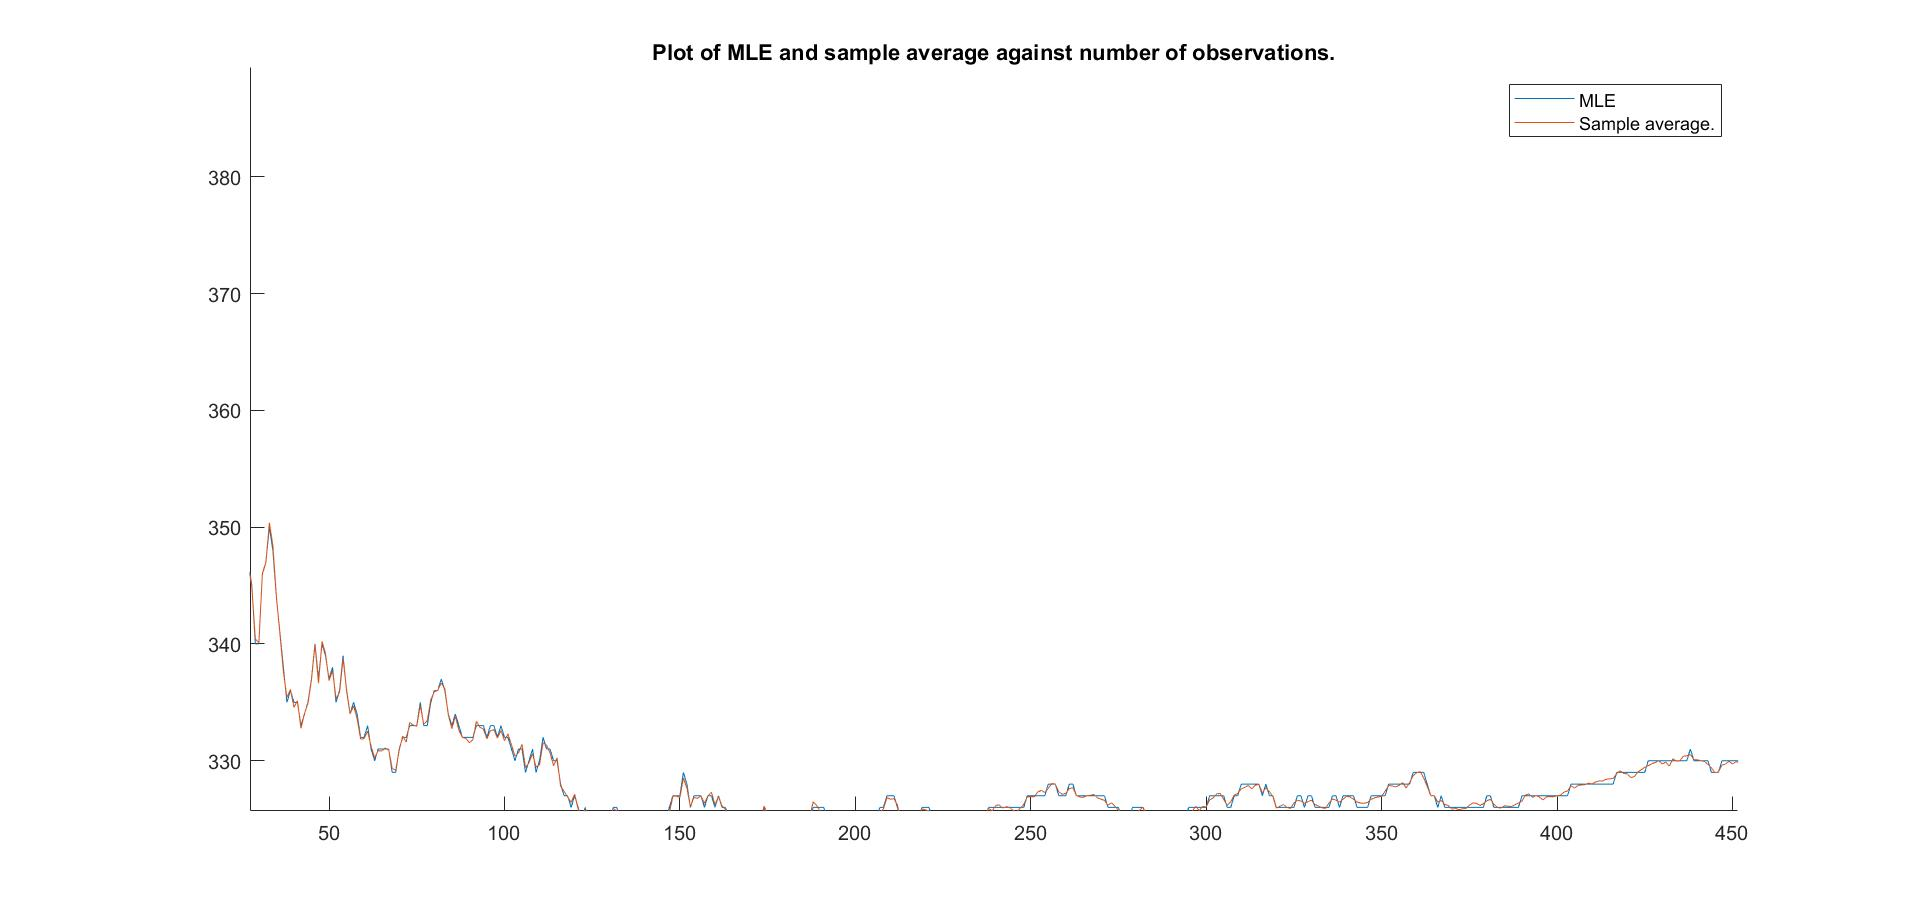
\includegraphics[width=13cm]{q10var100.jpg}
\caption{The estimators over a run of 1000 data points with variance 100.}
\label{fig:10v100}
\end{figure} 
\end{center}

\begin{center}
\begin{figure}[!htb]
\centering
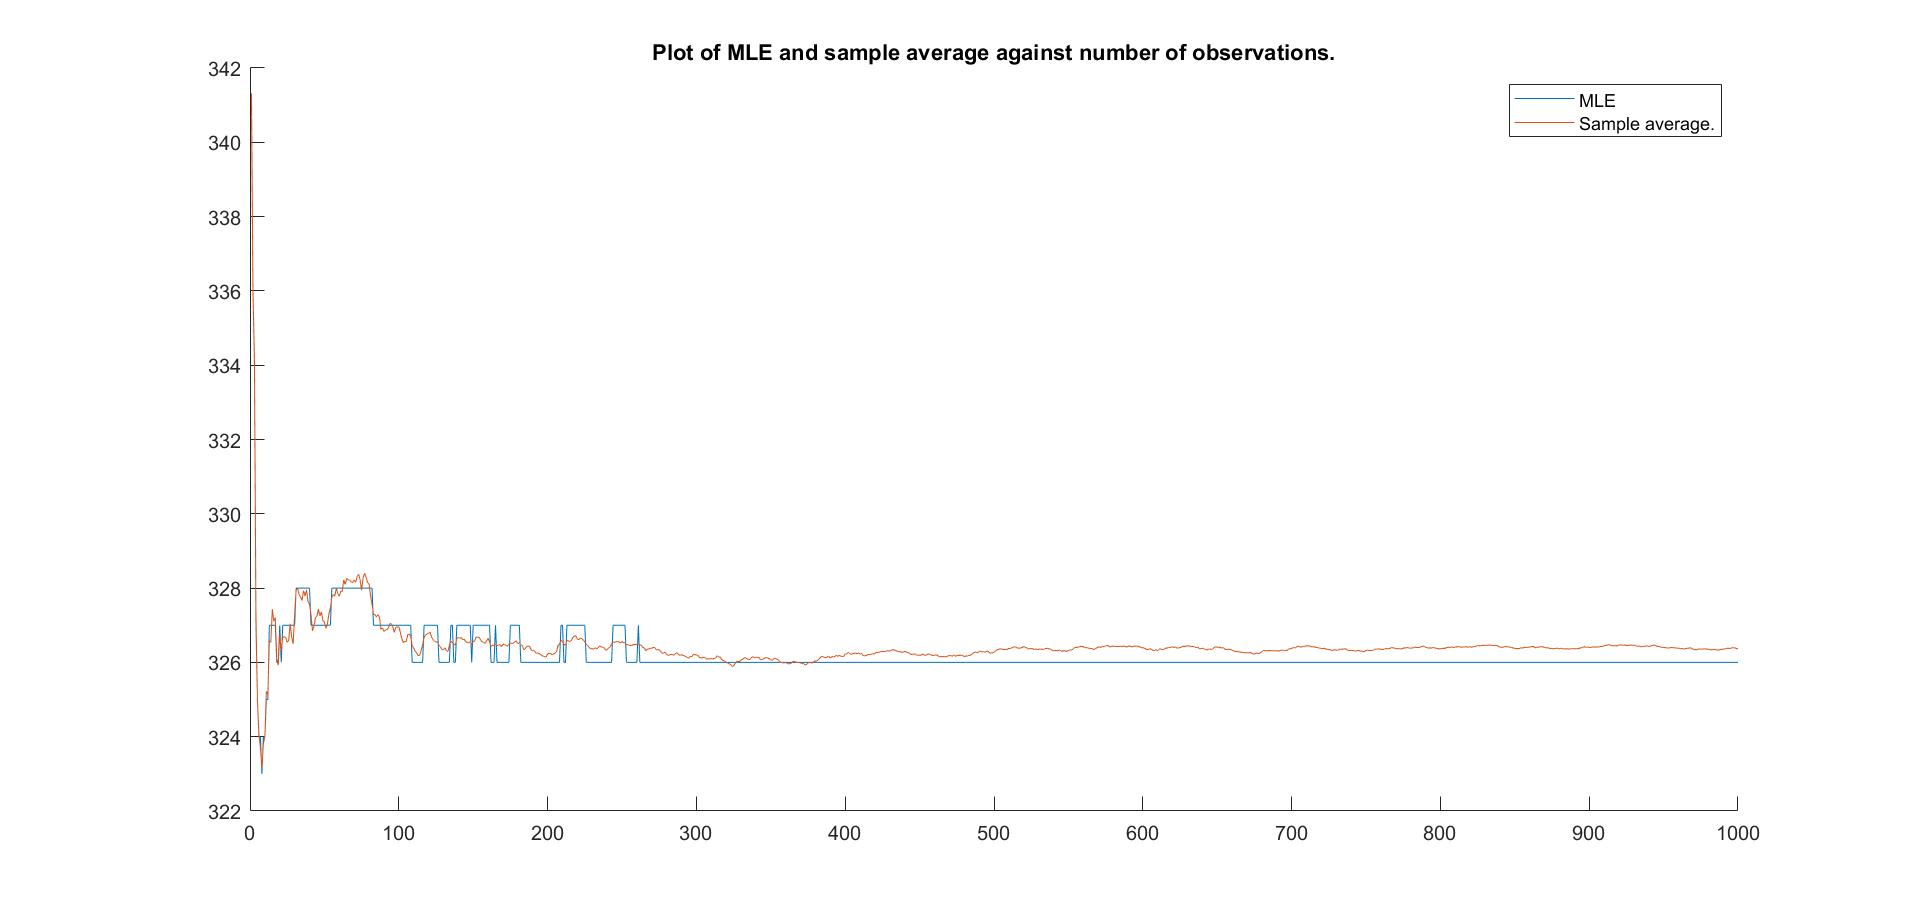
\includegraphics[width=13cm]{q10var10.jpg}
\caption{The estimators over a run of 10000 data points with variance 10.}
\label{fig:10v10}
\end{figure} 
\end{center}

\begin{center}
\begin{figure}
\centering
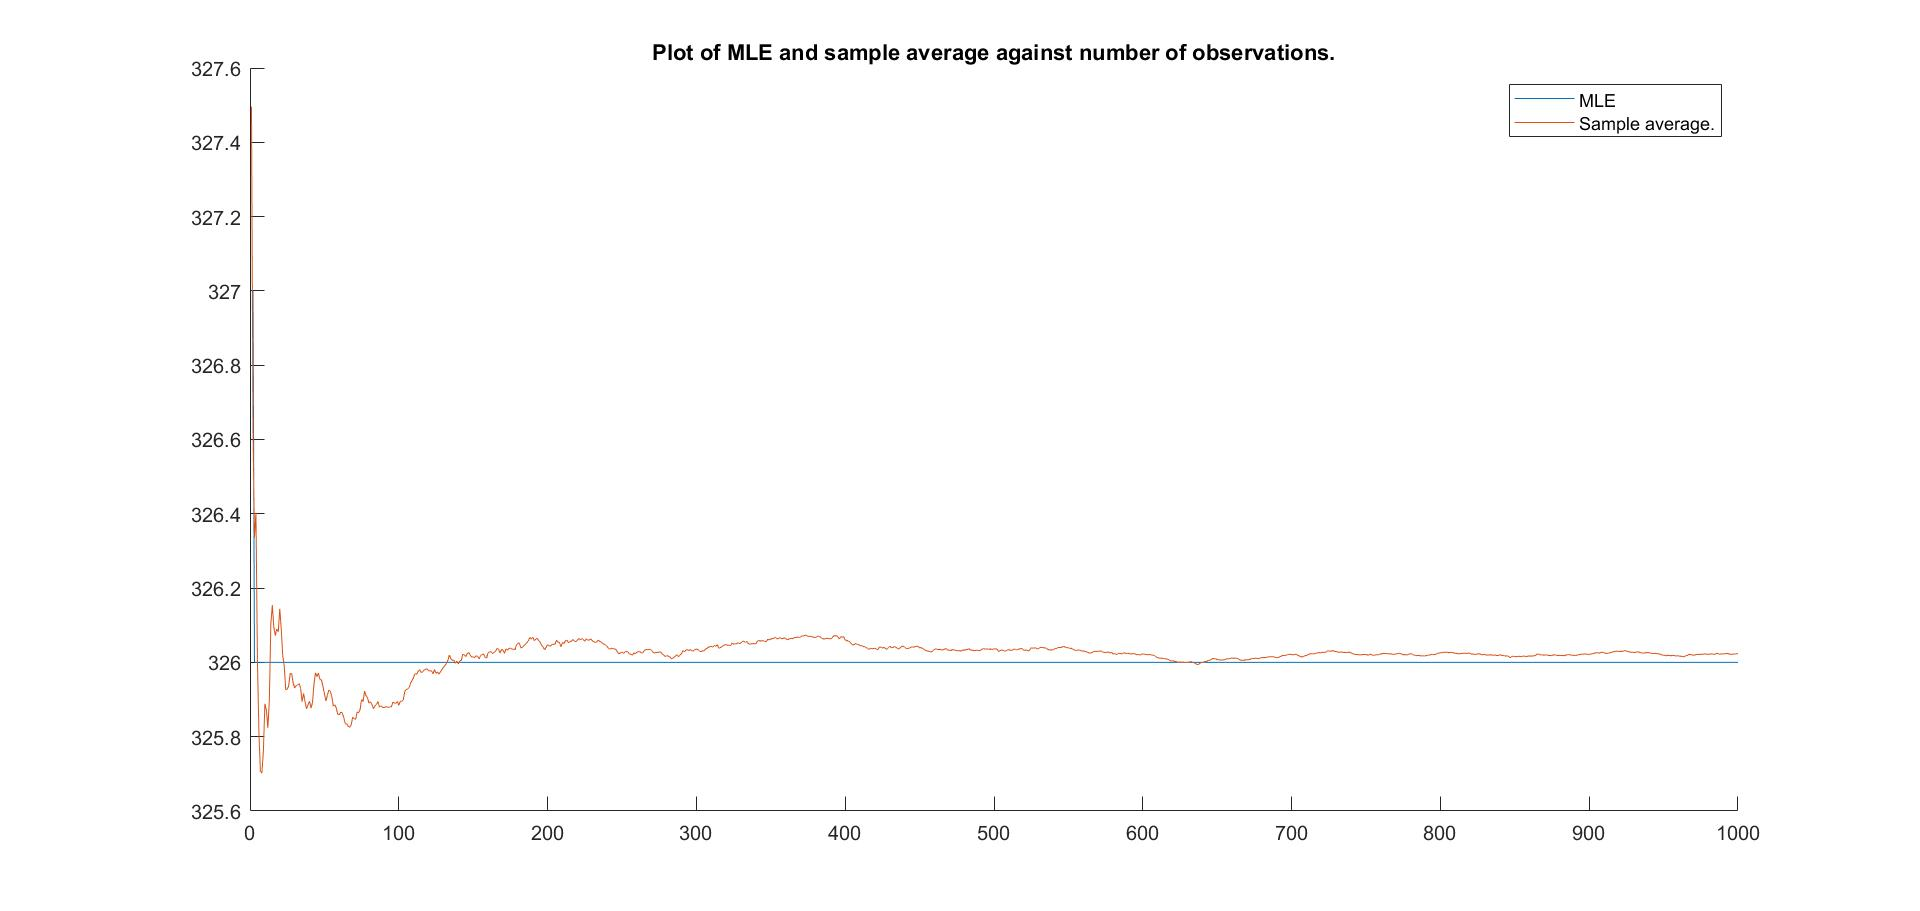
\includegraphics[width=13cm]{q10var1.jpg}
\caption{The estimators over a run of 1000 data points with variance 1.}
\label{fig:10v1}
\end{figure} 
\end{center}

For variance equal to 100, we find that the estimators in fact track each other very highly - the benefit of rounding the sample average is low when the variance disturbs the data enough. However, decreasing the variance to 10 indicates the advantages of the MLE, and decreasing to 1 shows immediate benefits to the estimator, indicating that if gaps between points in the parameter space are on the order of the variance, this method should be preferred. The simulation exercise would seem to to suggest that the coefficient $c$ in equation (\ref{eqn:rate}) is highly sensitive to the ratio of the variance and the spacing within the parameter space, as for higher variances, it's not at all clear that the performance is outperforming the sample average.





\clearpage
\bibliographystyle{siam}
\bibliography{references}






\end{document}